\section{DAGGER Implementation}
\begin{enumerate}
\item 
For collecting rollouts during training, we allow the simulation for the maximum number of timesteps allowed by the environment (or till failure).
\item Trajectories are collected will be have atleast a target number of timesteps (total), which are added to the buffer.
\item
At every timestep, give the current state of the agent (observation), the next action is chosen, with $\beta$ probability using the expert's policy, otherwise, the agent's policy.

\item Batch size number of observations are sampled from the buffer. The MLP predicts the actions on these, which are training against the expert's predictions on these observations using $\mathcal{L}_2$ loss.
\end{enumerate}

\section{Environment Description}
\begin{table}[H]
\centering
\begin{tabular}{lccc}
\hline
\textbf{Environment} &\textbf{Observation space}& \textbf{Action space} & {Action type} \\
&\textbf{dimension}& \textbf{dimension} &  \\
\hline
\texttt{Hopper-v4} & $11$ & $3$ & \texttt{continuous}\\
\texttt{Ant-v4}    & $27$ & $8$ & \texttt{continuous}\\
\hline
\end{tabular}
\caption{Environment Description}
\label{tab:environment_description}
\end{table}

\section{Best Model Evaluation Metrics}
\subsection{\texttt{Hopper-v4} Agent}
\begin{table}[H]
\centering
\begin{tabular}{lccccc}
\hline
\textbf{Agent} &
\texttt{n\_layers} &
\texttt{hidden\_size} &
\textbf{Episode mean} & \textbf{Episode mean} & \textbf{Episode stdev} \\
&
&
&
\textbf{length} &
\textbf{return} &
\textbf{return} \\
\hline
\texttt{Expert} & -  & - & $884-888$ & $2667-2676$ & $467-482$\\
\texttt{Imitation}  & $3$  & $64$ & $851.7$ & $2646.5$ & $631.6$\\
\texttt{Imitation*}  & $3$  & $128$ & $945.8$ & $2838.3$ & $377.0$\\
\texttt{Imitation}  & $3$  & $256$ & $953.0$ & $ 2873.9$ & $351.1$\\
\hline
\end{tabular}
\caption{\texttt{Hopper-v4} agent. Episode maximum length (set by environment) is $1000$, training rollouts sampled till $15,000$ timesteps collected, $30$ minutes of training on CPU,  $\beta = 0.1$, replay buffer size $50,000$, batch size $512$, \texttt{Adam(lr = 1e-3)} optimizer, model saving metric described in \nameref{sec:metric}. Evaluation over $1000$ trajectories.}
\label{tab:hopper-v4-metrics}
\end{table}
\subsection{\texttt{Ant-v4} Agent}
\begin{table}[H]
\centering
\begin{tabular}{lccccc}
\hline
\textbf{Agent} &
\texttt{n\_layers} &
\texttt{hidden\_size} &
\textbf{Episode mean} & \textbf{Episode mean} & \textbf{Episode stdev} \\
&
&
&
\textbf{length} &
\textbf{return} &
\textbf{return} \\
\hline
\texttt{Expert} & -  & - & $999-1000$ & $1009-1027$ & $260-285$\\
\texttt{Imitation}  & $4$  & $128$ & $1000.0$ & $969.8$ & $2.7$\\
\texttt{Imitation}  & $4$  & $256$ & $1000.0$ & $938.9$ & $5.0$\\
\texttt{Imitation*} & $5$  & $128$ & $1000.0$ & $977.0$ & $2.9$\\
\texttt{Imitation}  & $5$  & $256$ & $1000.0$ & $943.8$ & $2.1$\\
\hline
\end{tabular}
\caption{\texttt{Ant-v4} agent. Episode maximum length (set by environment) is $1000$, training rollouts sampled till $15,000$ timesteps collected, $60$ minutes of training on CPU,  $\beta = 0.1$, replay buffer size $50,000$, batch size $512$, \texttt{Adam(lr = 1e-3)} optimizer, model saving metric described in \nameref{sec:metric}. Evaluation over $1000$ trajectories.}
\label{tab:ant-v4-metrics}
\end{table}
\section{Metric for model saving}\label{sec:metric}
\begin{table}[H]
\centering
\begin{tabular}{cl}
\hline
\textbf{Environment} & \textbf{Reward} \\
\hline
\texttt{Hopper-v4} & \texttt{healthy\_reward + forward\_reward - ctrl\_cost} \\
\texttt{Ant-v4} & \texttt{healthy\_reward + forward\_reward - ctrl\_cost - contact\_cost} \\
\hline
\end{tabular}
\caption{Reward functions for different environments}
\label{tab:rward_model}
\end{table}
From \autoref{tab:rward_model} we see that the reward is a proxy for the episode length in both cases (\texttt{forward\_reward} component). Hence we track the evaluation return, instead of episode length. Since evaluation is done on only around $15$ trajectories, we use the metric
\begin{equation*}
    \texttt{metric = eval\_mean\_return - eval\_stdev\_return}
\end{equation*}
This intends to maximize the "worst performance" of the agent. To make this requirement even harder, the coefficient of \texttt{eval\_stdev\_return} can be increased, for example   \texttt{metric = eval\_mean\_return - 3 * eval\_stdev\_return}.


\section{Observations}
\begin{enumerate}
\item As evident in the training plots below (\texttt{Ant-v4}), the model doesn't get trained well and the return keeps reducing.
Since the \texttt{Ant-v4} agent is 4-legged, it doesn't fall and hence the episode length is usually $1000$ (full episode). \item Even without training the policy network (\texttt{n\_layers = 2, hidden\_size = 64}), the average episode length is $1000$ and for return, mean $957$ with standard deviation $12$.
\item We suspect this is because the return is mostly dominated by \texttt{forward\_reward}, which always reaches it's full value, and there's not enough room left to learn skill. 

\item We tried experimenting with reducing learning rate, \autoref{fig:ant-small-lr} but the return just \textbf{reduces} more slowly in this case. Similarly, changing \texttt{min\_timesteps\_per\_batch} too didn't help.
\end{enumerate}


\begin{figure}[H]
\centering
\begin{minipage}{0.45\textwidth}
    \centering
    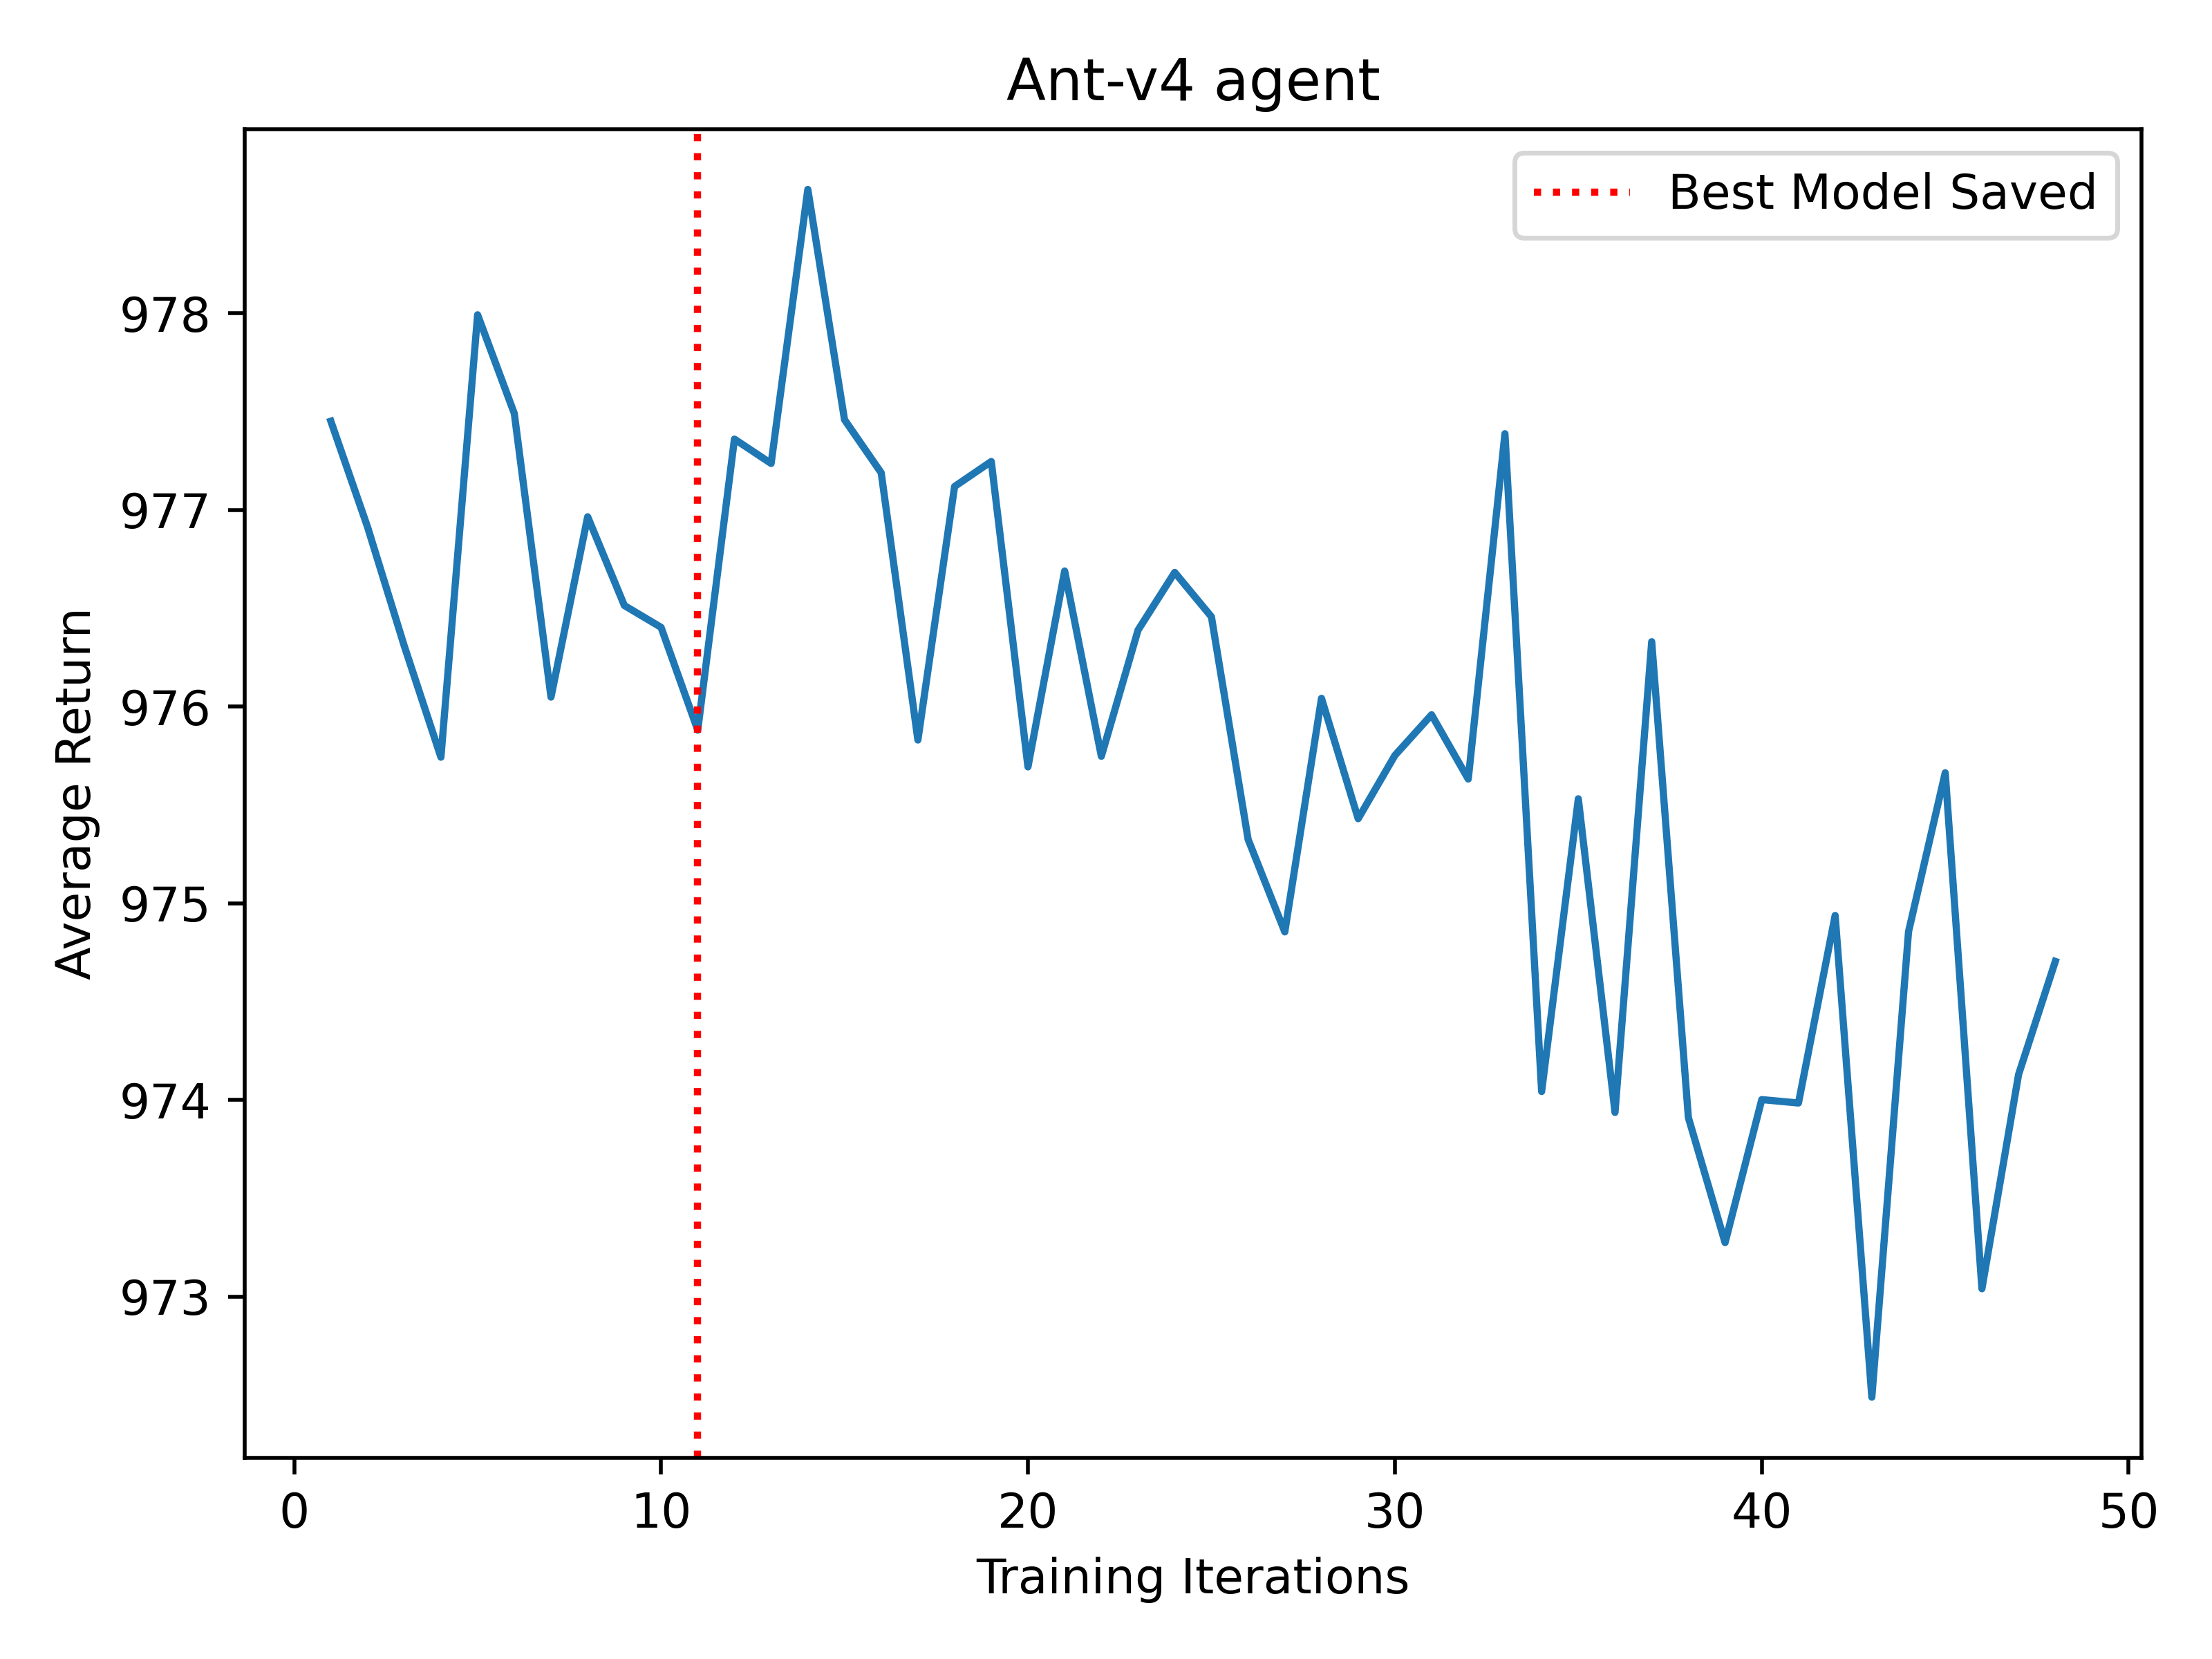
\includegraphics[width=\linewidth]{plots/Ant-v4_avg_return-small-lr.png}
    \caption*{Average Return}
\end{minipage}
\hspace{0.02\textwidth}
\begin{minipage}{0.45\textwidth}
    \centering
    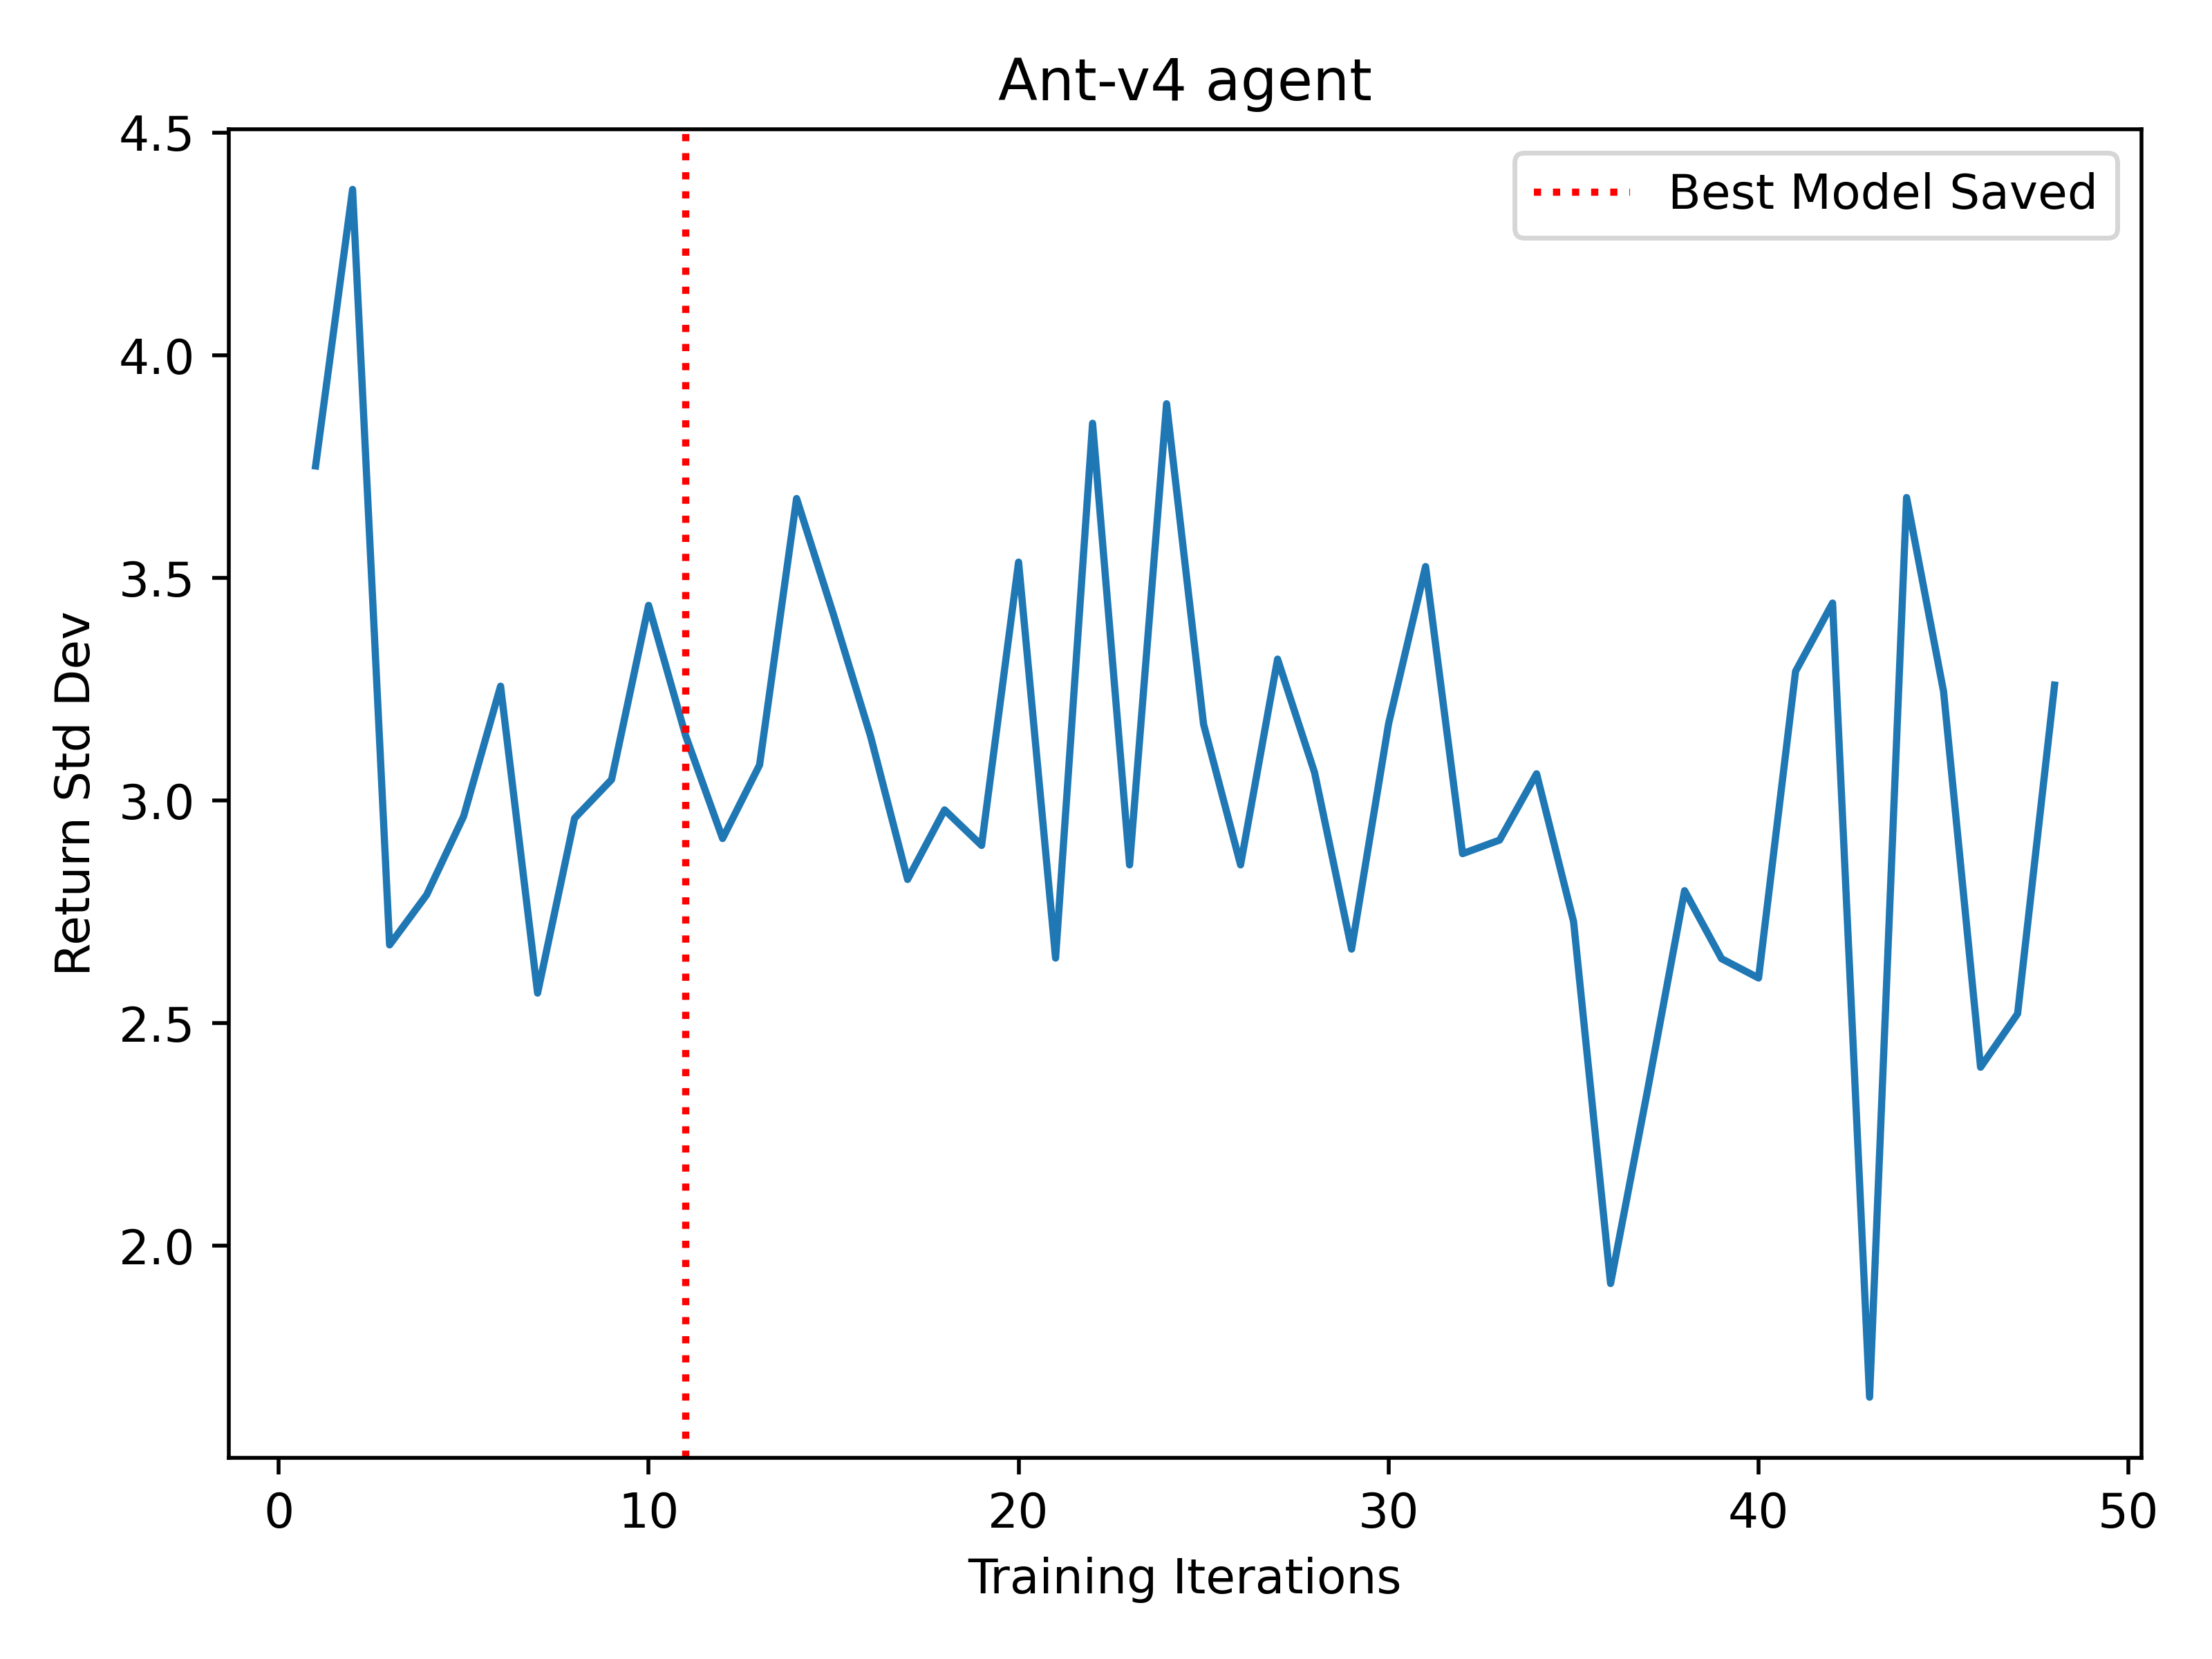
\includegraphics[width=\linewidth]{plots/Ant-v4_std_return-small-lr.png}
    \caption*{Standard Deviation of Return}
\end{minipage}
\caption{Evaluation metrics of \texttt{Ant-v4} agent with \texttt{lr = 1e-4}}
\label{fig:ant-small-lr}
\end{figure}


\section{Training Plots}

\begin{figure}[H]
\centering
\captionsetup{font=small}
\setlength{\belowcaptionskip}{-8pt}

% Row 1
\begin{minipage}{0.42\textwidth}
    \centering
    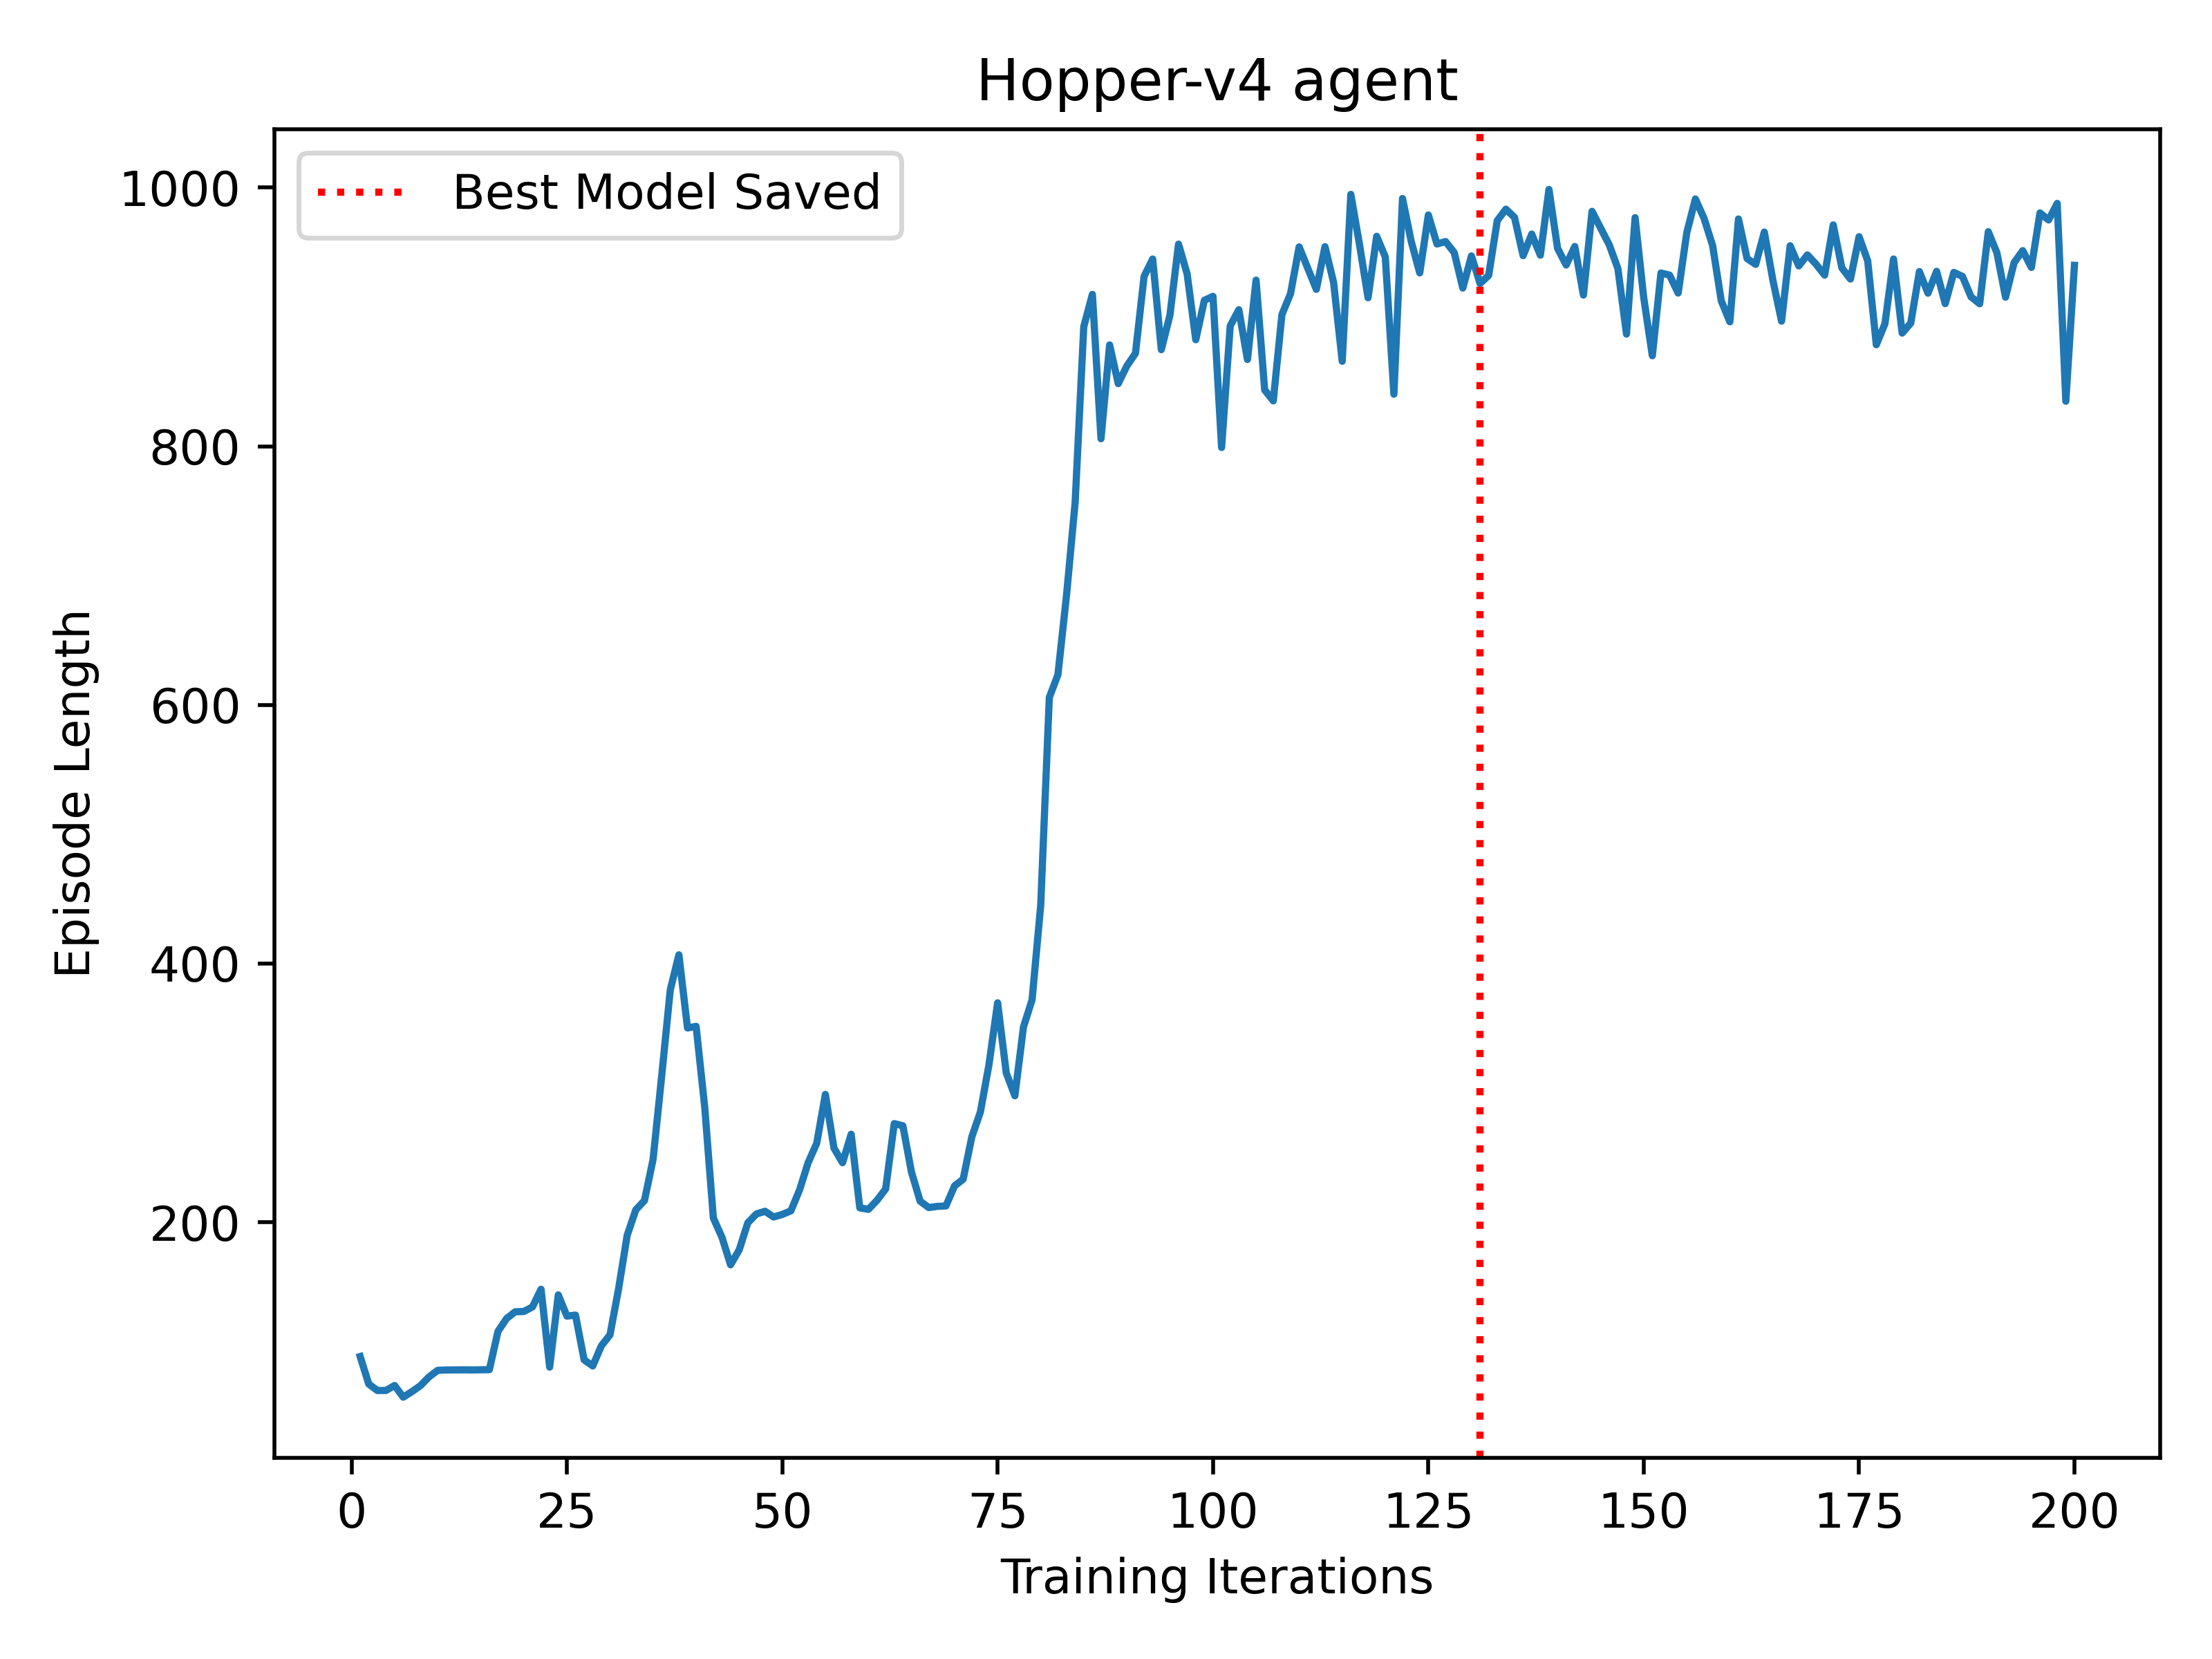
\includegraphics[width=\linewidth]{plots/Hopper-v4_episode_length.png}
\end{minipage}%
\hfill
\begin{minipage}{0.42\textwidth}
    \centering
    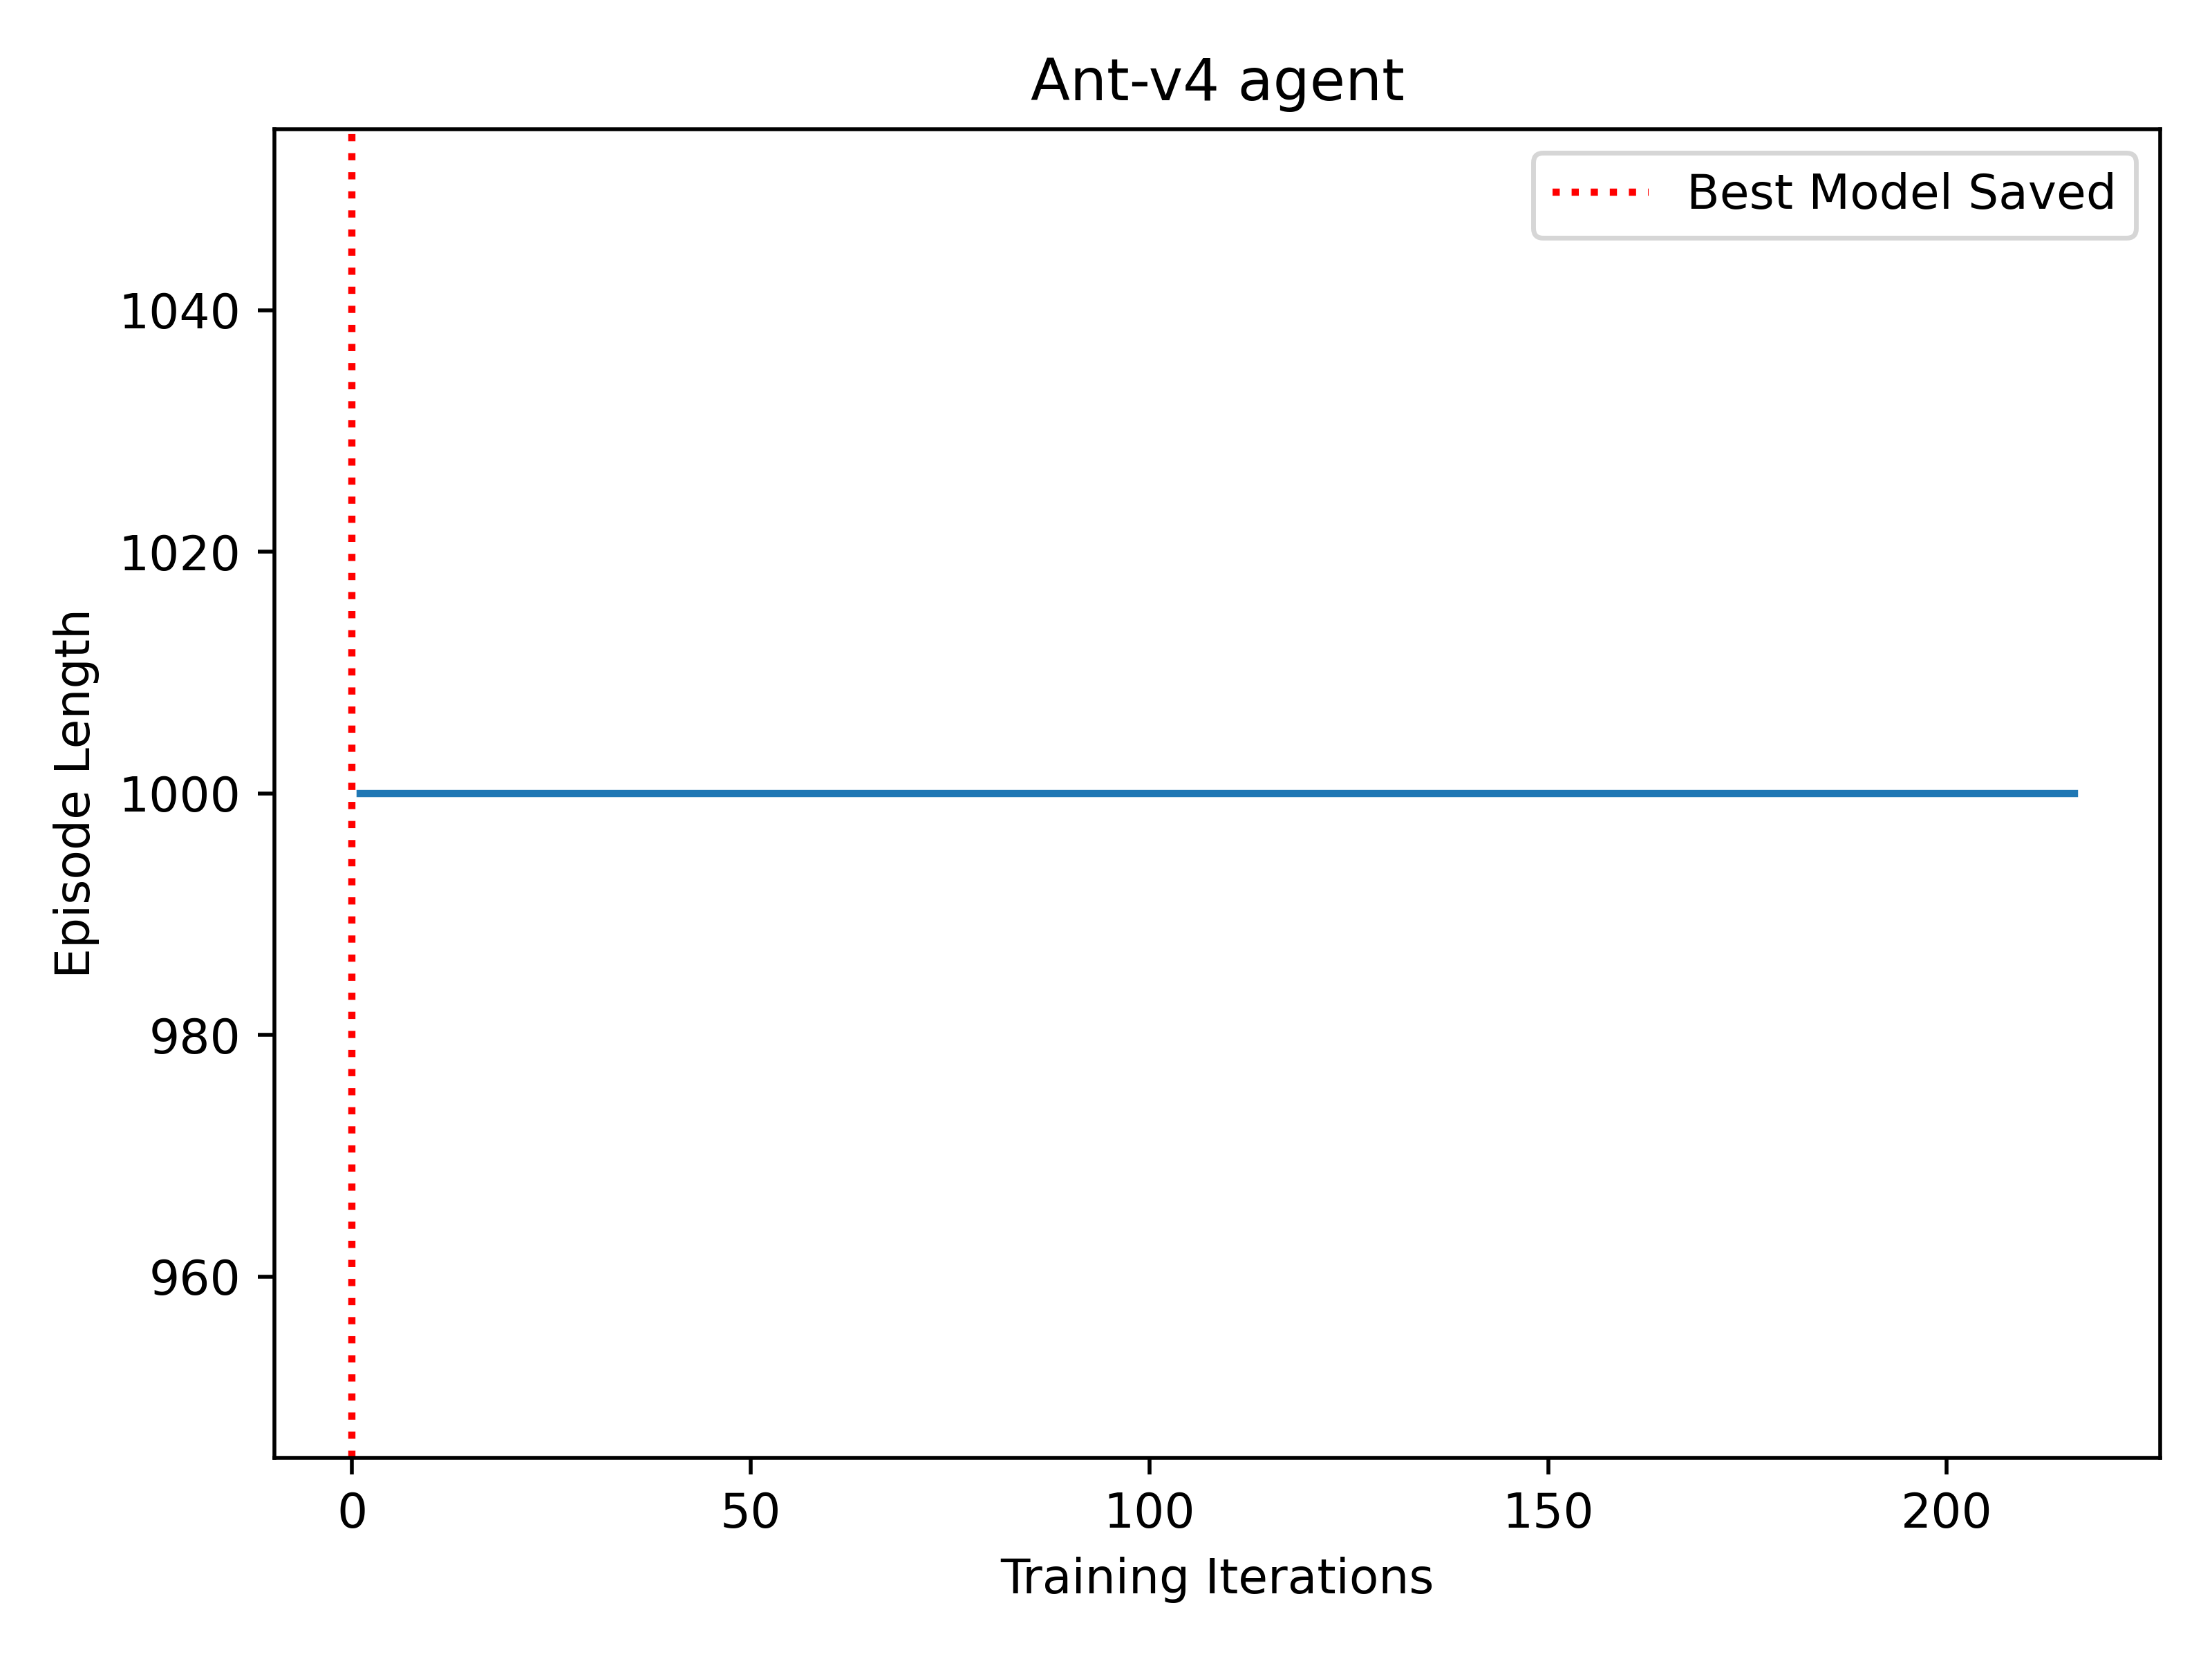
\includegraphics[width=\linewidth]{plots/Ant-v4_episode_length.png}
\end{minipage}

\vspace{0.25ex}

% Row 2
\begin{minipage}{0.42\textwidth}
    \centering
    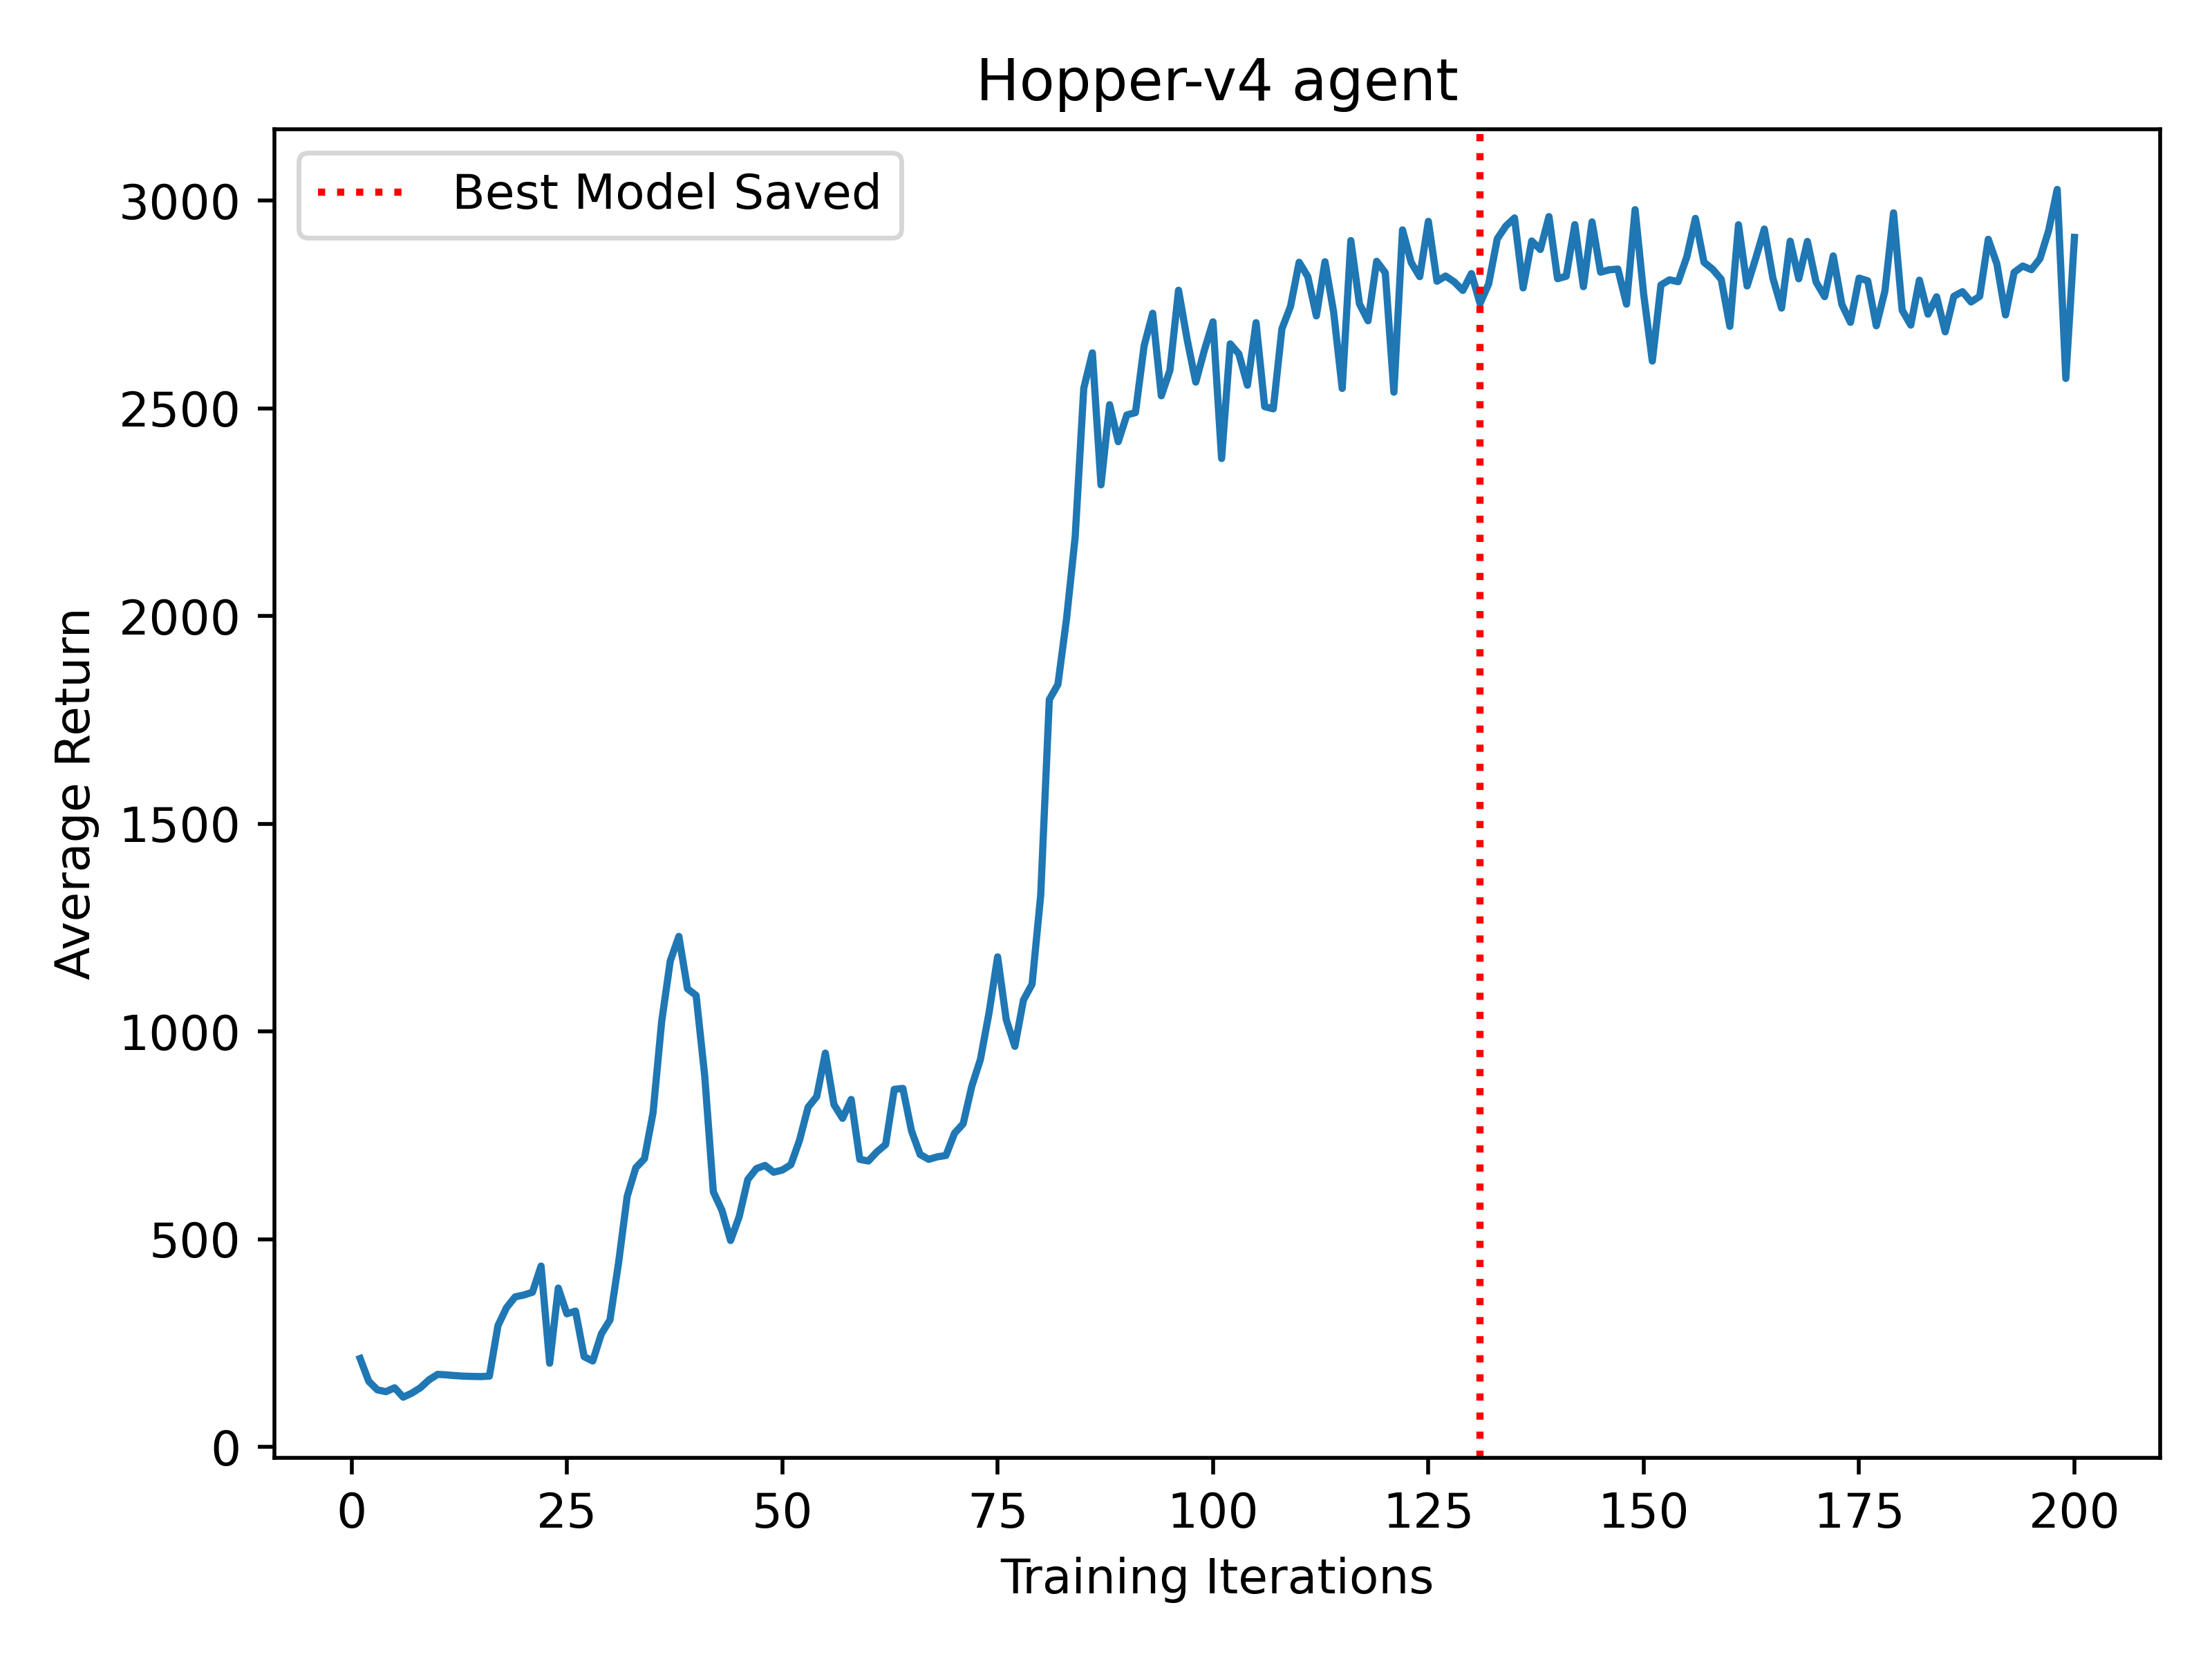
\includegraphics[width=\linewidth]{plots/Hopper-v4_avg_return.png}
\end{minipage}%
\hfill
\begin{minipage}{0.42\textwidth}
    \centering
    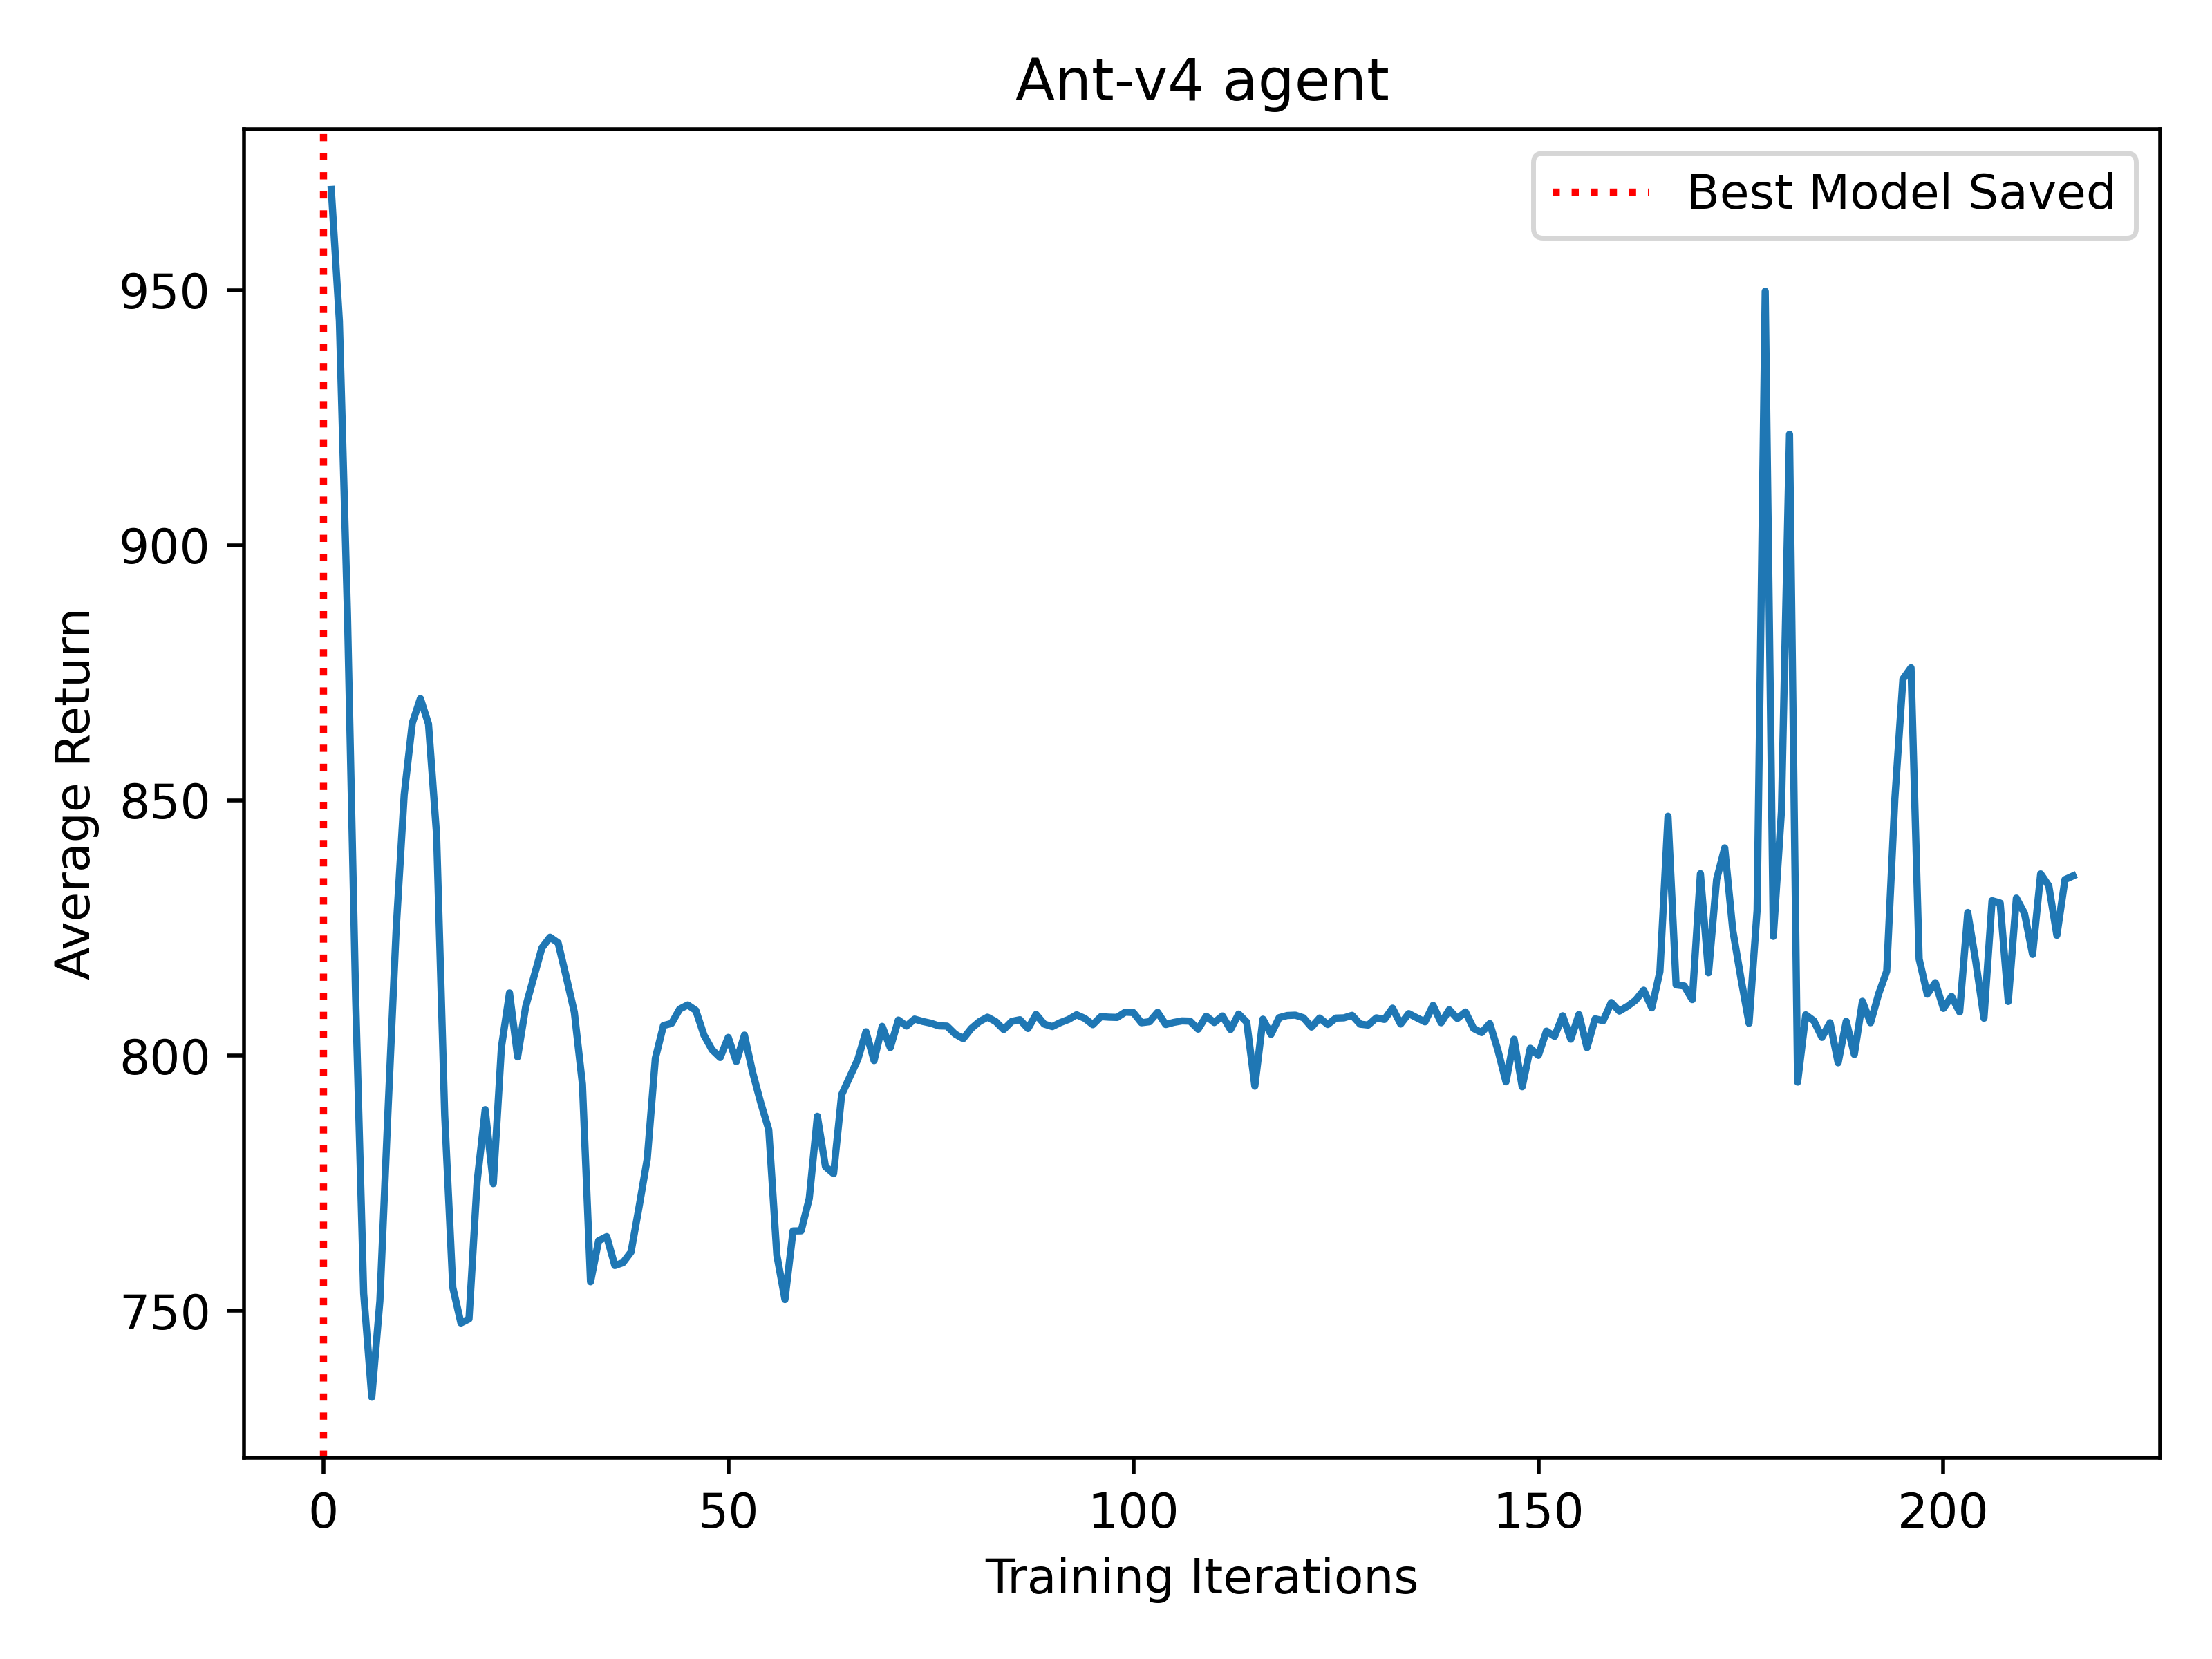
\includegraphics[width=\linewidth]{plots/Ant-v4_avg_return.png}
\end{minipage}

\vspace{0.25ex}

% Row 3
\begin{minipage}{0.42\textwidth}
    \centering
    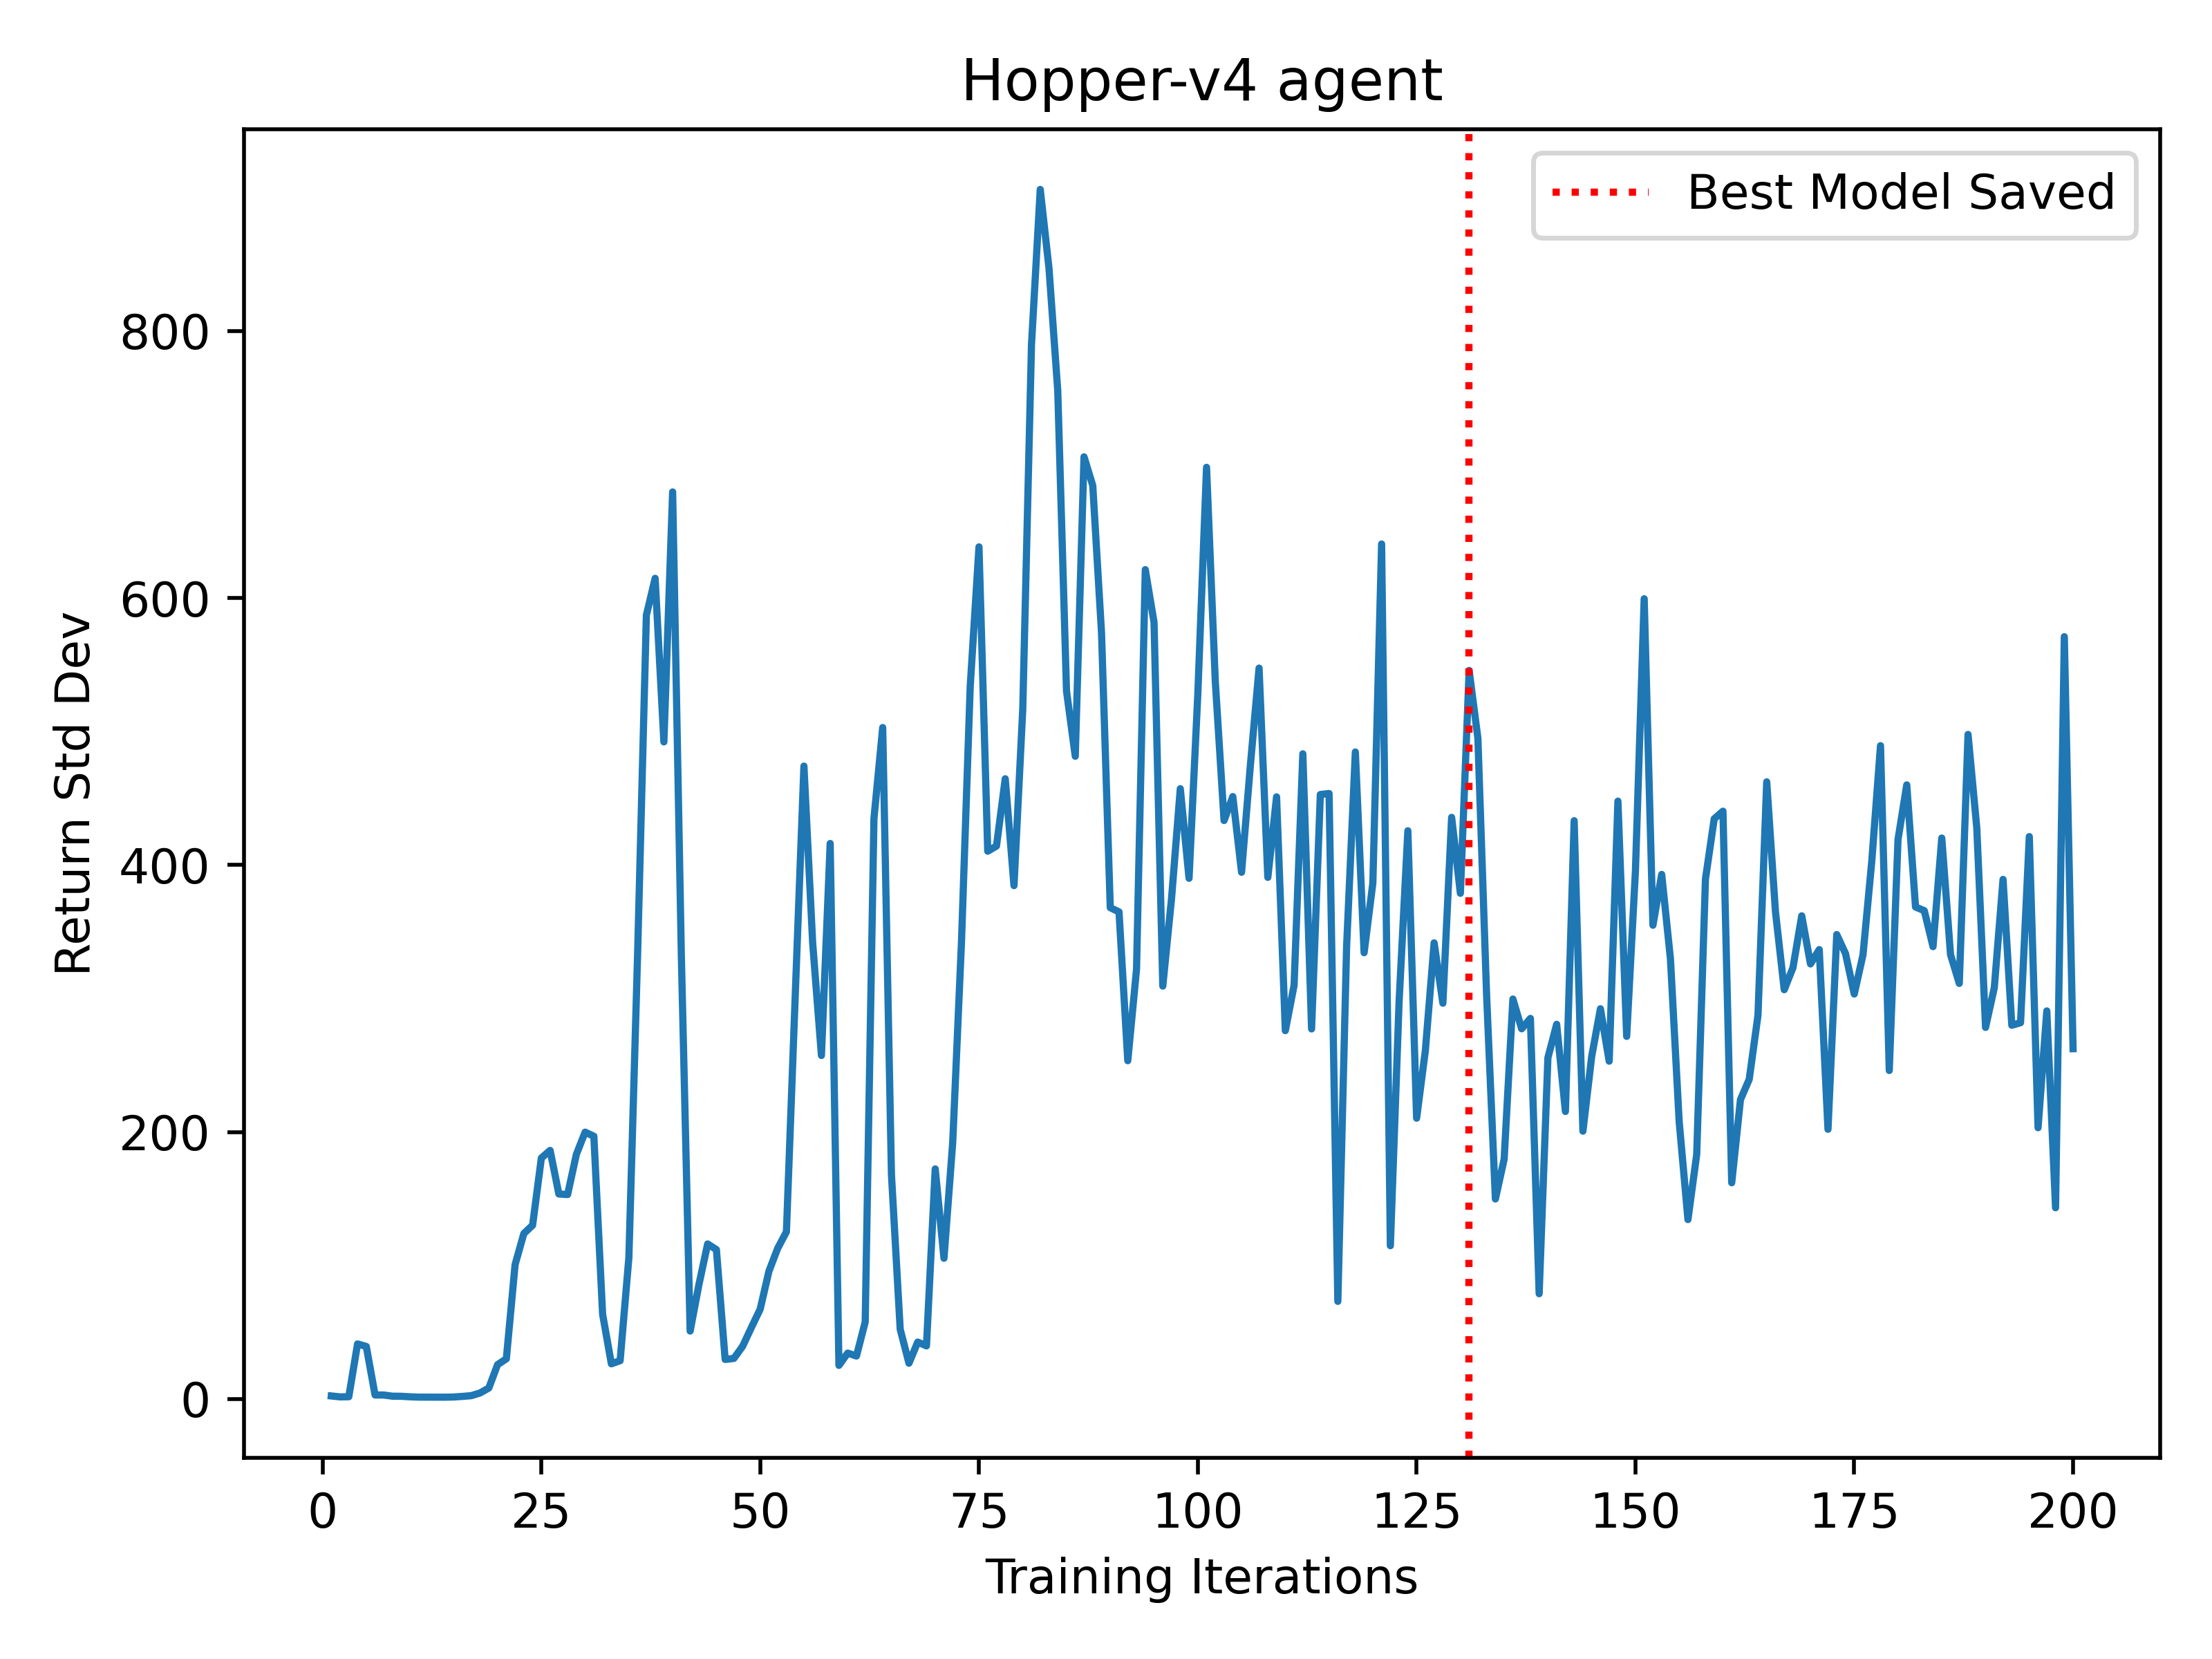
\includegraphics[width=\linewidth]{plots/Hopper-v4_std_return.png}
\end{minipage}%
\hfill
\begin{minipage}{0.42\textwidth}
    \centering
    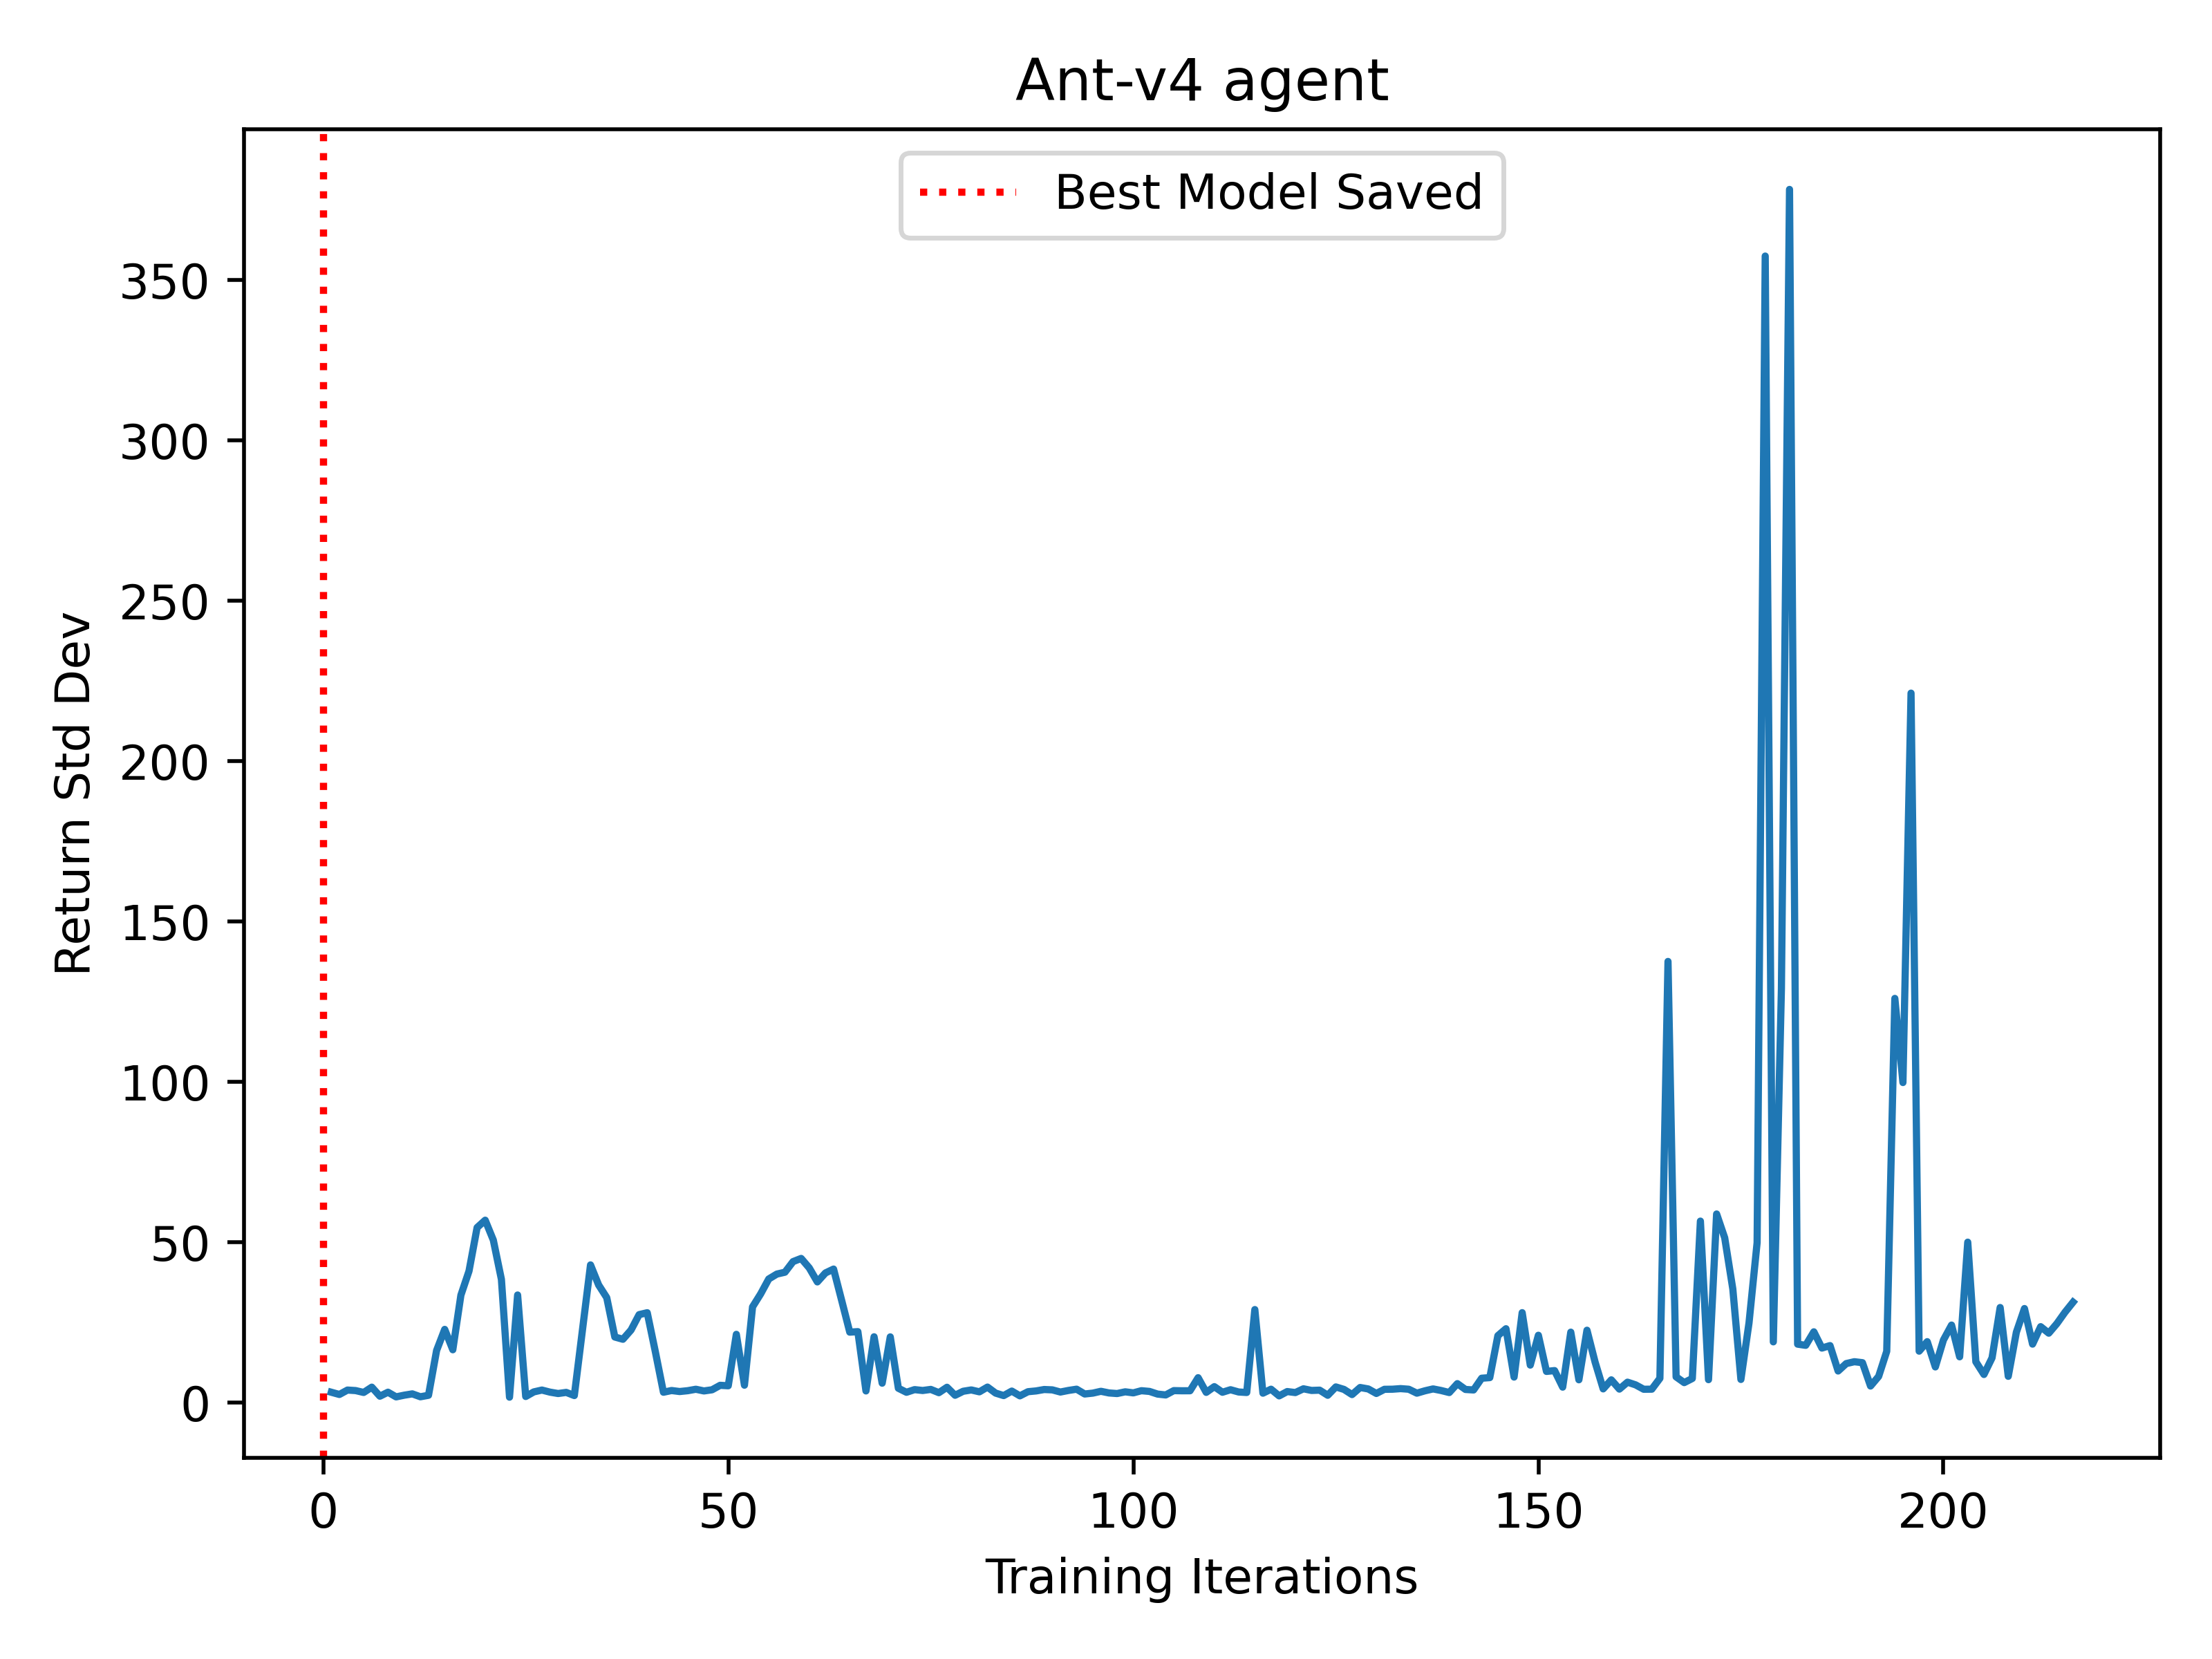
\includegraphics[width=\linewidth]{plots/Ant-v4_std_return.png}
\end{minipage}

\vspace{0.25ex}

% Row 4
\begin{minipage}{0.42\textwidth}
    \centering
    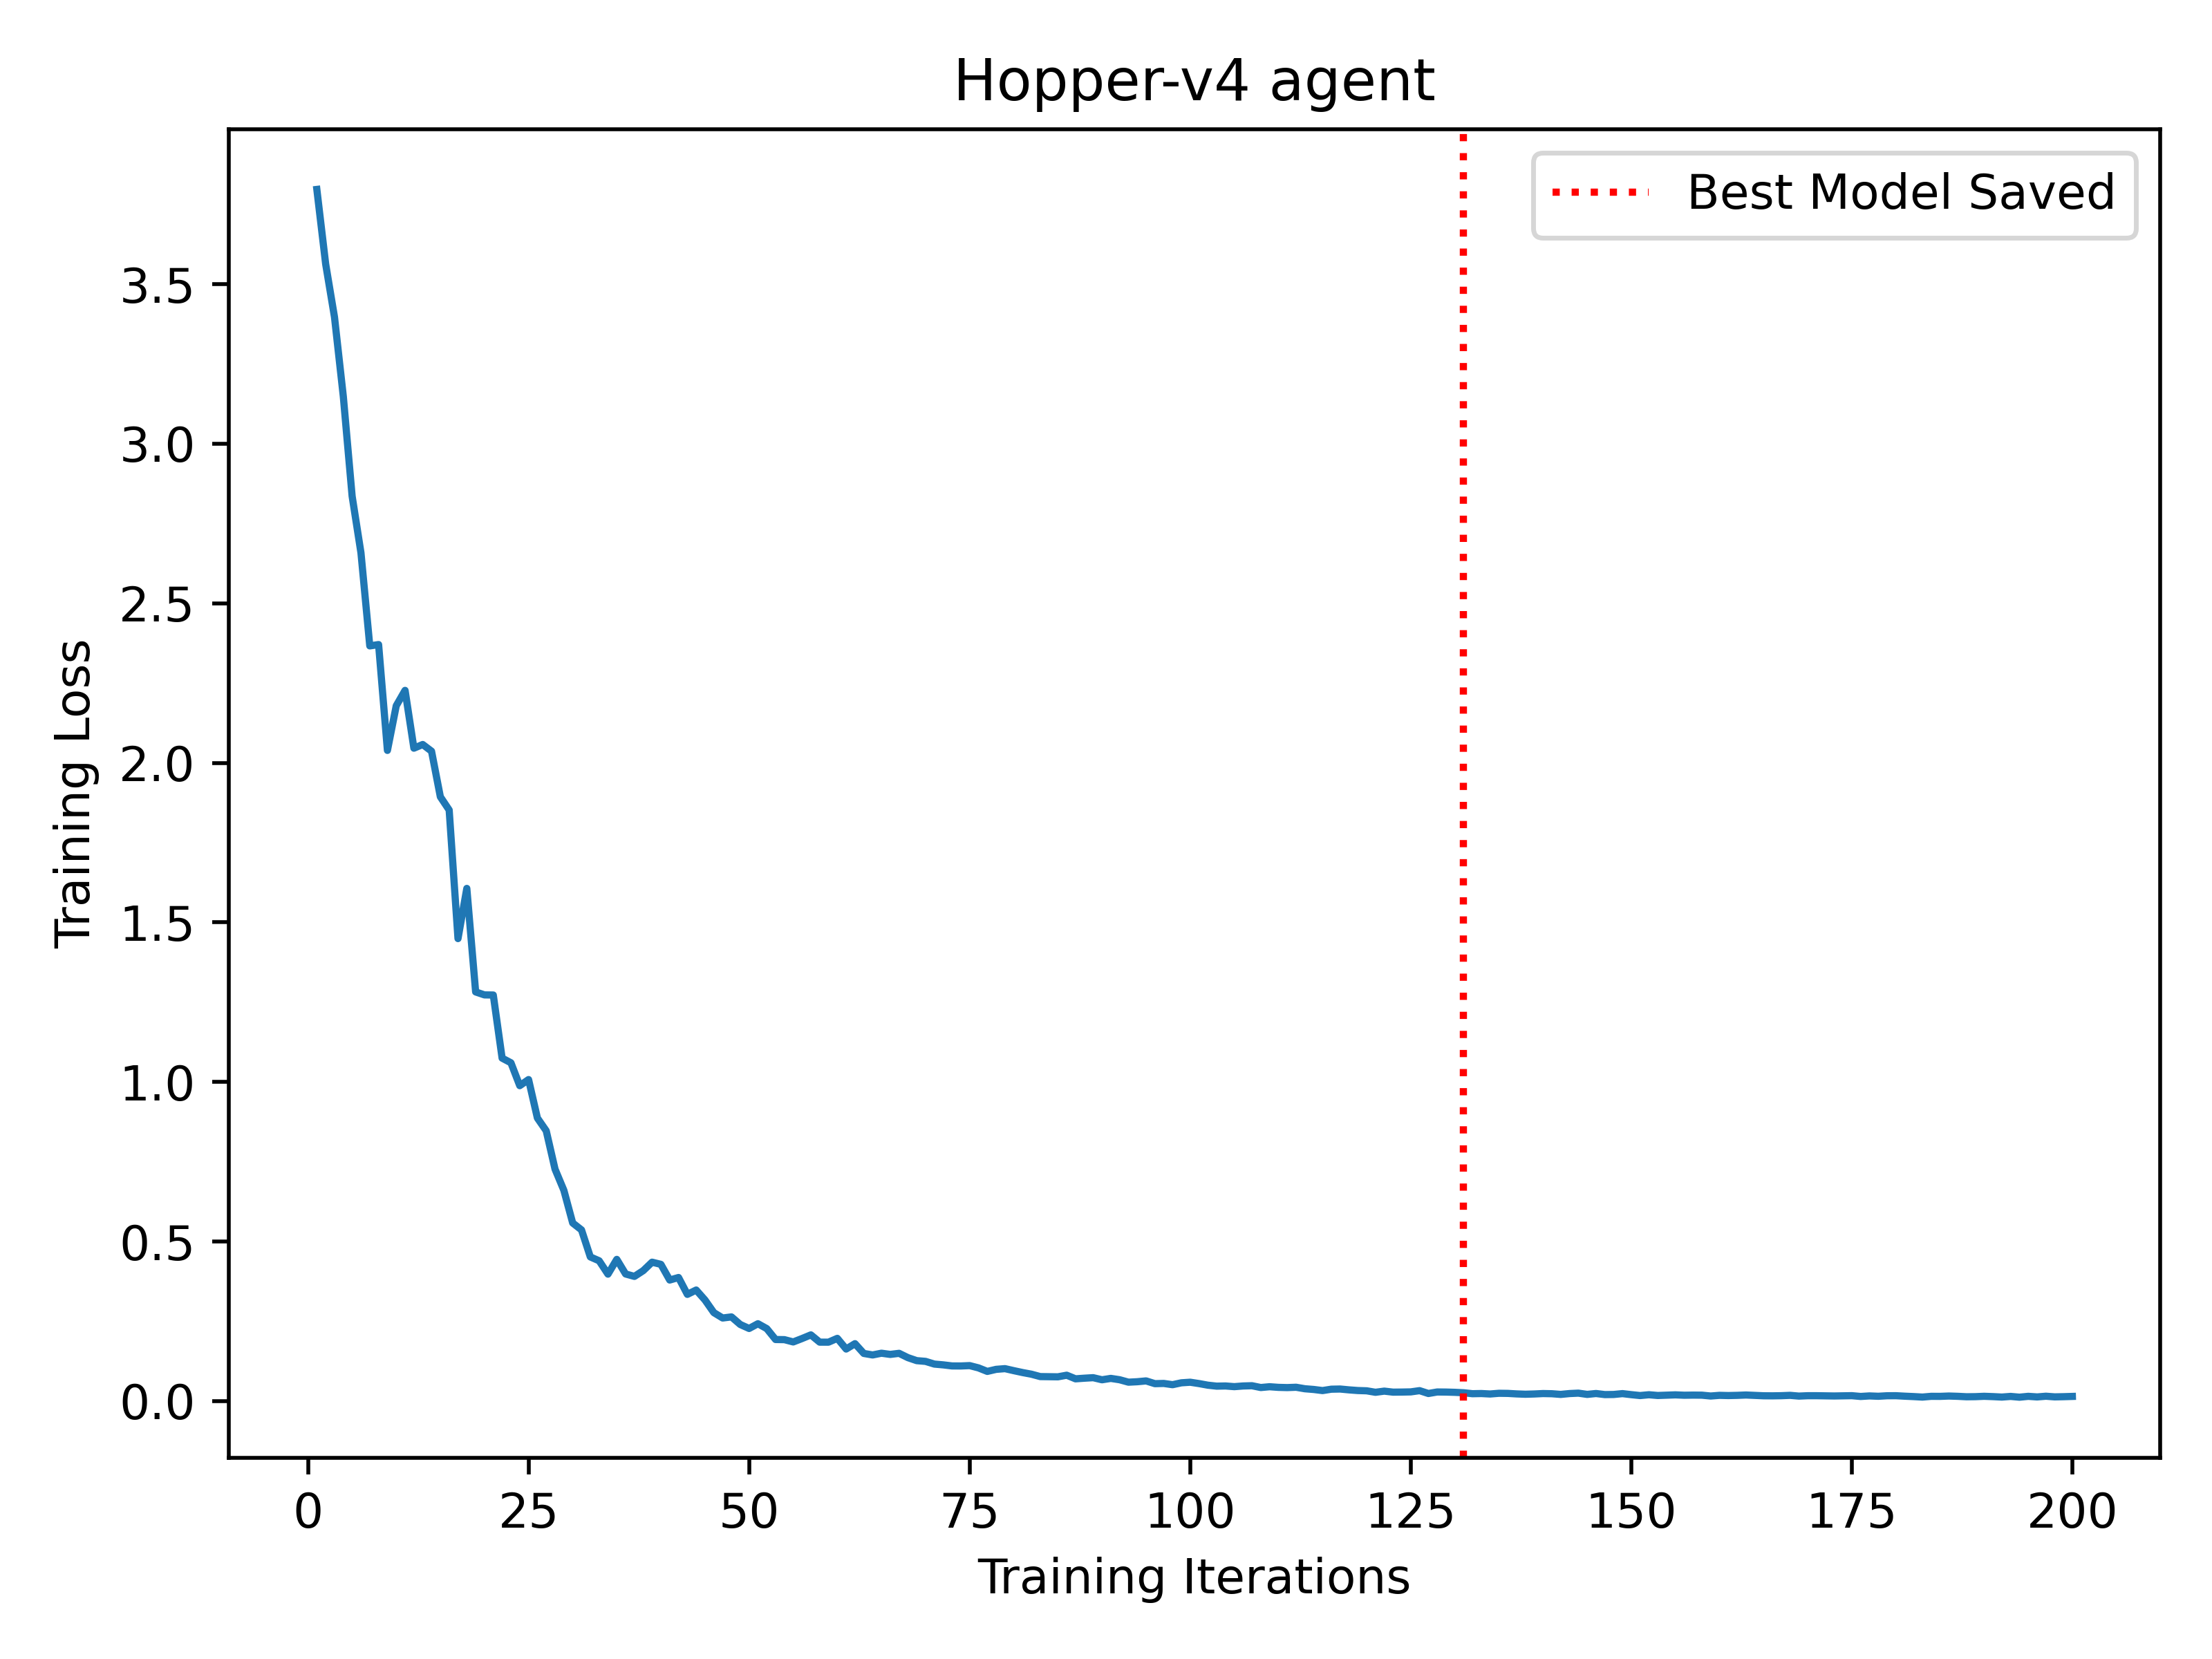
\includegraphics[width=\linewidth]{plots/Hopper-v4_train_loss.png}
\end{minipage}%
\hfill
\begin{minipage}{0.42\textwidth}
    \centering
    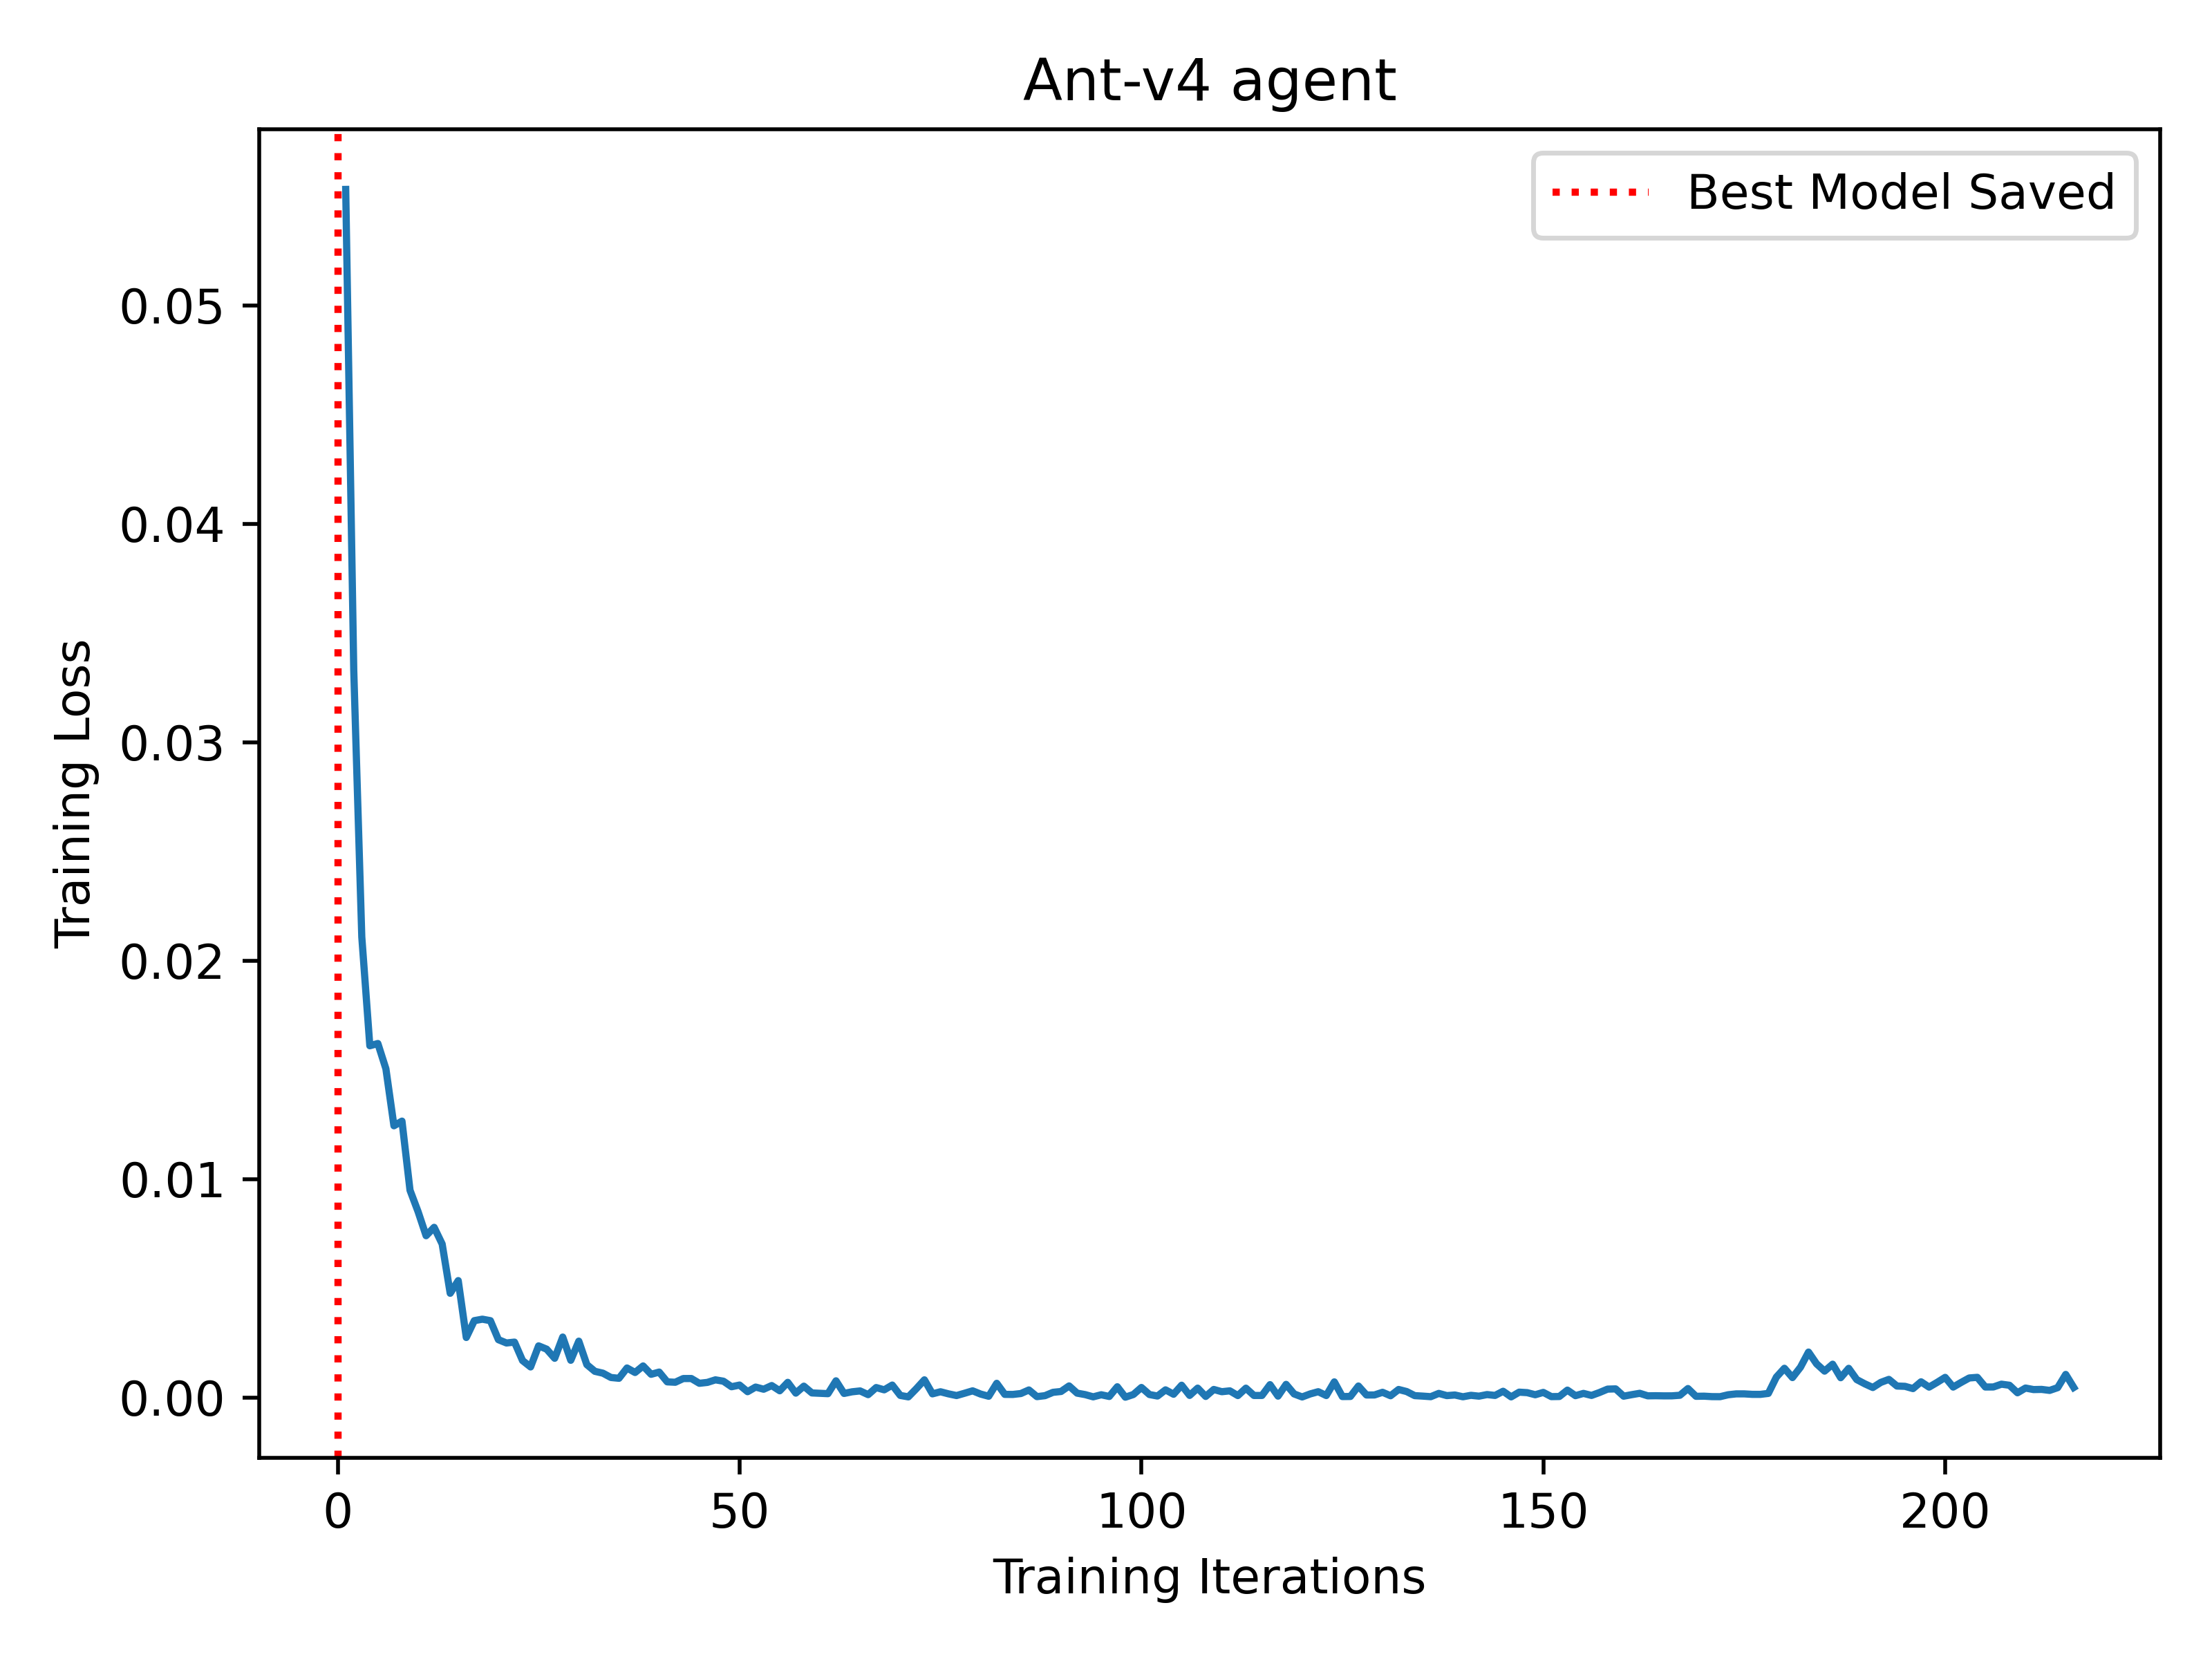
\includegraphics[width=\linewidth]{plots/Ant-v4_train_loss.png}
\end{minipage}

\caption{Evaluation metric while training. Mean Episode Length, Mean Return, Standard Deviation of Return, Training Loss (top to bottom). \texttt{Hopper-v4} (left), \texttt{Ant-v4} (right). Red dotted line indicates best-model.}
\end{figure}
